\pdfoutput=1
\documentclass[preprint,11pt]{elsarticle}
\usepackage[T1]{fontenc}
\usepackage[utf8]{inputenc}
\usepackage{lmodern,microtype}
\usepackage[a4paper,margin=23mm]{geometry}
\usepackage{amsmath,amssymb,amsthm}
\usepackage{graphicx,booktabs,tabularx,array,xcolor}
\usepackage{enumitem,caption,placeins,float,pifont}

\usepackage[colorlinks=true,linkcolor=black,citecolor=black,urlcolor=blue]{hyperref}
\usepackage{orcidlink}
\hypersetup{pdftitle={Mapping the Unseen: What an LLM API Can and Cannot Reveal About Its Architecture},pdfauthor={Abhyuday Patel, Ranjan Kumar Behera, Aditi Kumari, Pratik Chourasia}}
\definecolor{accent}{HTML}{E8604C}
\definecolor{ink}{HTML}{25231F}
\definecolor{soft}{HTML}{777167}
\definecolor{pale}{HTML}{F7F5F1}
\definecolor{okgreen}{HTML}{527F65}
\definecolor{missred}{HTML}{B66355}
\captionsetup{font=small,labelfont=bf,labelsep=period}
\setlist{nosep,leftmargin=1.4em}
\setlength{\emergencystretch}{3em}
\setlength{\tabcolsep}{4pt}
\renewcommand{\arraystretch}{1.15}
\renewcommand{\topfraction}{0.94}
\renewcommand{\bottomfraction}{0.85}
\renewcommand{\textfraction}{0.05}
\renewcommand{\floatpagefraction}{0.75}
\newcolumntype{Y}{>{\raggedright\arraybackslash}X}
\newtheorem{definition}{Definition}
\newtheorem{proposition}{Proposition}
\newcommand{\lvl}[1]{\textsf{#1}}
\newcommand{\yes}{{\color{okgreen}\ding{51}}}
\newcommand{\no}{{\color{missred}\ding{55}}}
\newcommand{\unknown}{\textsf{U}}
\newcommand{\benchname}{ForensicsBench}
\renewcommand{\paragraph}[1]{\par\smallskip\noindent\textit{#1}\quad}
\makeatletter
\let\ps@pprintTitle\ps@plain
\makeatother
\newcommand{\BenchN}{26}
\newcommand{\BenchNScored}{25}
\newcommand{\ProtocolHash}{31fc86fdc7fa99a8}
\newcommand{\ContractAcc}{25/25}
\newcommand{\TokenizerAcc}{18/24 exact; 5 correct abstentions; 1 wrong}
\newcommand{\TokenizerExactN}{18}
\newcommand{\FamilyPathAcc}{25/25}
\newcommand{\SsmSplitAcc}{8/8 decided (11 abstained)}
\newcommand{\SsmEligible}{19}
\newcommand{\SsmNA}{2}
\newcommand{\BenchEncoders}{4}
\newcommand{\DtypeAcc}{80\% (25 subjects)}
\newcommand{\MoeAcc}{88\%}
\newcommand{\AttnRefAcc}{90\%}
\newcommand{\AttnFlatAcc}{38\%}
\newcommand{\BenchArchs}{20}
\newcommand{\BenchClusters}{21}
\newcommand{\BenchECEMacroCI}{[0.153, 0.351]}
\newcommand{\BenchBrierMacroCI}{[0.272, 0.429]}
\newcommand{\BenchECEMacroLegacyCI}{[0.153, 0.346]}
\newcommand{\BenchBrierMacroLegacyCI}{[0.269, 0.423]}
\newcommand{\BenchECE}{0.249}
\newcommand{\BenchBrier}{0.348}
\newcommand{\BenchECELegacy}{0.244}
\newcommand{\BenchBrierLegacy}{0.344}
\newcommand{\GeomResolvedAcc}{15/15}
\newcommand{\GeomMaxWidth}{2,048}
\newcommand{\GeomMaxErr}{2.6\%}
\newcommand{\GeomMedErr}{0.00\%}
\newcommand{\GeomResolvedList}{128, 256, 512, 576, 768, 896, 1024, 2048}
\newcommand{\GeomArtifacts}{gpt2-int8: rank 57 vs true 768; gpt2-wirebf16: rank 2552 vs true 768; router-gpt2-pythia: rank 1474 vs true 768}
\newcommand{\TopFiveCols}{6}
\newcommand{\WitnessPrompts}{48}
\newcommand{\WitnessRank}{764 vs true 768/1024}
\newcommand{\KappaTiming}{2.02}
\newcommand{\KappaTimingCI}{[1.85, 103.41]}
\newcommand{\KappaTimingReq}{1.3}
\newcommand{\KappaTok}{0.0177}
\newcommand{\KappaTokCI}{---}
\newcommand{\KappaTokReq}{150}
\newcommand{\KappaWire}{deterministic grid}
\newcommand{\KappaWireCI}{---}
\newcommand{\KappaWireReq}{O(1)}
\newcommand{\JevSecrets}{10}
\newcommand{\JevStateEff}{+0.98}
\newcommand{\JevSibEff}{+0.00}
\newcommand{\JevPermP}{2\times10^{-4}}
\newcommand{\DsFreshExp}{0.57}
\newcommand{\DsFreshCI}{[0.41, 0.74]}
\newcommand{\DsFreshN}{56}
\newcommand{\DsRepeatExp}{0.22}
\newcommand{\DsRepeatCI}{[0.04, 0.40]}
\newcommand{\DsRepeatN}{21}
\newcommand{\GptFreshExp}{0.17}
\newcommand{\GptFreshCI}{[-0.01, 0.36]}
\newcommand{\PlannerSeeds}{8}
\newcommand{\PlannerStaticDecisive}{150}
\newcommand{\PlannerEigDecisive}{185}
\newcommand{\PlannerUniformDecisive}{233}
\newcommand{\PlannerMoeEig}{188}
\newcommand{\PlannerMoeStatic}{151}
\newcommand{\BlindN}{48}
\newcommand{\BlindCap}{100\%}
\newcommand{\BlindLedger}{100\%}
\newcommand{\BlindRound}{100\%}
\newcommand{\BlindSwap}{100\%}
\newcommand{\BlindRouter}{100\%}
\newcommand{\BlindNone}{100\%}
\newcommand{\NVWidthResolved}{0/25}
\newcommand{\NVDepthErr}{30\%}
\newcommand{\LLMmapIdent}{71\%}
\newcommand{\LLMmapFam}{35\%}


\begin{document}
\begin{frontmatter}
\title{\textbf{Mapping the Unseen:\\[2pt] What an LLM API Can and Cannot Reveal About Its Architecture}}
\author[1]{Abhyuday Patel\,\orcidlink{0009-0006-5898-2395}\corref{cor1}}
\ead{abhyuday.2023ug4002@iiitranchi.ac.in}
\cortext[cor1]{Corresponding author}
\author[1]{Ranjan Kumar Behera}
\ead{ranjan@iiitranchi.ac.in}
\author[2]{Aditi Kumari}
\ead{aditikumarikv4@gmail.com}
\author[1]{Pratik Chourasia}
\ead{pratik.2023ug2051@iiitranchi.ac.in}
\affiliation[1]{organization={Indian Institute of Information Technology, Ranchi},country={India}}
\affiliation[2]{organization={Jamshedpur Women's University},country={India}}
\begin{abstract}
What can an API tell you about the hidden system behind it?  Most answers to that
question are guesses.  Ours is a measurement.  We treat the problem as
\emph{functional architecture identification under partial observability}.  In plain
words: we ask which parts of a model's design can be worked out from the outside,
through the API alone, and which parts cannot.  Then we measure that boundary instead
of reporting one best-guess architecture.  The answer splits into four kinds of
property.  Some are \emph{identifiable}: the API contract, the tokenizer's count
family, the autoregressive-compatible generation contract, the width of the output
bottleneck over a measured range, and the numeric grid of the values sent over the
wire.  Some are \emph{cost-limited}: they can be separated in principle, and we
\emph{estimate} how much information each request buys on each channel (a per-channel
discrimination density $\hat\kappa$) to say how many requests the job needs under the
stated probe family.  Some are \emph{access-limited}: the API simply hides the channel
we would need, as with top-5-only logprobs for width, buffered streaming for decode
timing, and depth.  And some are \emph{provably non-identifiable}: we give two scoped
equivalence witnesses, and we build one of them for real, a width-768 model and a
width-1024 twin with zero observable difference.  The instrument is an active probe
library with an evidence-ranking engine.  The measuring stick is \benchname{}, a blind
ground-truth benchmark that serves \BenchN{} known models (dense transformers, Mamba
SSMs, mixture-of-experts, MLA, encoders, and an encoder-decoder, with dtype, batching,
and router variants) behind one anonymous contract with frozen thresholds.  On this
ground truth the battery recovers the API contract (\ContractAcc), the tokenizer
count-family (\TokenizerAcc), the autoregressive-compatible generation contract
(\FamilyPathAcc), the transformer-vs-SSM split (\SsmSplitAcc{} of \SsmEligible{}
eligible subjects, through a validated decode-state probe), the output-bottleneck width
over a measured range (resolved through \GeomMaxWidth{}, with lower bounds at the
acquisition limit and never over-resolved), and the wire grid (\DtypeAcc).  It is weak
on MoE (\MoeAcc) and blind to depth, and the theory says why each hole exists.  The
same battery then reconstructs GPT-4o-mini, DeepSeek-V3.2, and the JEV decision
endpoint, with every component graded by the reliability its detector earned on ground
truth.  Baselines in the style of NightVision and LLMmap run on the same subjects.  A
live multi-seed planner study and a commit-reveal blind fixture suite complete the
evaluation.  The contribution is the measured identification boundary
$[\omega]_{\mathcal C,\mathcal X}$, not a claim of exact model reverse engineering.
\end{abstract}
\begin{keyword}
functional architecture identification \sep black-box forensics \sep system
identification \sep identifiability \sep language-model serving \sep active probing
\end{keyword}
\end{frontmatter}

\noindent\small\textbf{Companion artifact.} Scanner, \benchname{} harness and journals,
frozen protocol, and reproduction scripts:
\url{https://github.com/AbhyudayPatel/mapping-the-unseen}
\normalsize

\section{Introduction}
\label{sec:intro}
Frontier models are rented, not downloaded.  You send a request to an API and an answer
comes back.  The weights stay hidden.  But the API is not a blank wall.  Every answer is
produced by a real pipeline: a tokenizer, an embedding table, a stack of attention or
state-space blocks, an output projection, and a serving system wrapped around all of
it.  Each of these stages leaves small traces in what comes back: the token counts on
the bill, the score vectors (logprobs), the timing, and the way errors are reported.
This paper asks one quantitative question and answers it with a measurement:
\begin{quote}
\textbf{What can an API reveal about a hidden computational system?  Exactly how much of
its functional architecture can be identified, and where does identification provably
stop?}
\end{quote}

The answer is not a yes or a no.  It is a \emph{four-way boundary}.  Some properties
are \textbf{identified} outright by sending controlled requests.  Some are
\textbf{cost-limited}: they can be separated in principle, but each request buys only a
little evidence, so the real question is how many requests the job needs.  We answer
that with an estimate of the information one request carries, written $\hat\kappa$,
under a stated family of probes.  Some are \textbf{access-limited}: the API does not
expose the channel at all.  Top-5-only logprobs, buffered streams, and a deployment cap
are all examples.  And some are \textbf{non-identifiable}: two different architectures
provably produce identical observations, and we show the pair explicitly.  In formal
terms, what we recover is the \emph{equivalence class} $[\omega]_{\mathcal C,\mathcal
X}$, the set of all configurations that would look identical through the channels we
have, and, for each property $g$, the \emph{identified set} $\mathcal
I_g(\omega;\mathcal C,\mathcal X)$, the values of that property that remain possible.
We never recover the literal configuration $\omega$, and we do not pretend to.

\begin{figure}[t]\centering
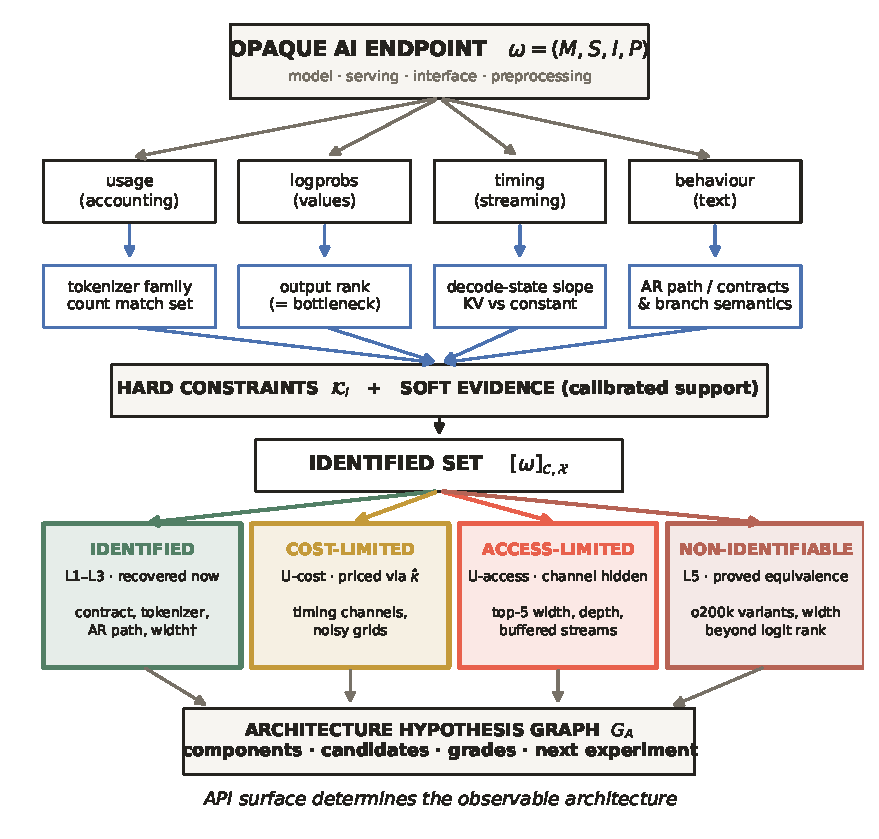
\includegraphics[width=.8\textwidth]{figures/fig_v4_masterflow.pdf}
\caption{The whole paper on one page.  An opaque endpoint $\omega=(M,S,I,P)$ is probed
through four kinds of channel: usage accounting, logprobs, timing, and behaviour.
Each observation becomes either a hard constraint or a piece of graded soft evidence.
Together they define the identified set $[\omega]_{\mathcal C,\mathcal X}$, which sorts
every component into one of four classes: identified, cost-limited, access-limited, or
witnessed non-identifiable.  What remains is the architecture hypothesis graph $G_A$: an
honest reconstruction, with a grade and a named next experiment attached to every
node.}
\label{fig:masterflow}
\end{figure}

\begin{table}[t]\centering\small
\caption{The identification boundary, measured.  Left: the functional components the
battery identifies, with accuracy measured on \benchname{} (known models served behind an
anonymous API, with detector thresholds frozen in advance).  Right: the components that
stay open, each with the reason.  The reason is always one of three things: a proved
equivalence witness (grade L5), a channel whose per-request information $\kappa$ we have
estimated, or a named next experiment.  Production rows are graded by how reliable the
detector proved on the benchmark, never simply asserted.}
\label{tab:boundary}
\begin{tabularx}{\textwidth}{@{}Y c Y@{}}
\toprule
\textbf{Identified (with measured accuracy)} & \textbf{Bench} & \textbf{Open, and why}\\
\midrule
API contract and serving limits & \ContractAcc & depth: compute and queueing are tangled
together; identity-layer witness (App.~A)\\
Tokenizer count-family \& template overhead & \TokenizerAcc & exact vocabulary: the
reference set has gaps (DeepSeek: 465 unresolved entries)\\
AR-compatible generation contract vs encoder readout & \FamilyPathAcc & ---\\
Transformer vs constant-state (SSM) split & \SsmSplitAcc & production span limit: decode
growth is drowned in noise at $\le$12k context (U-cost)\\
Output bottleneck width $d$ (rich access) & \GeomResolvedAcc & top-5-only access: rank
$\le$ a handful of columns (witness, Prop.~\ref{prop:rank})\\
Wire numeric grid (fp32/bf16/fp16) & \DtypeAcc & internal compute dtype: transport rounding
hides it\\
Dense vs MoE feed-forward & \MoeAcc & weakest detector; production claims discounted
to match (Sec.~\ref{sec:production})\\
Decision branch/readout structure (JEV) & $p=\JevPermP$ & physical prefill sharing:
only the operator can attest it\\
\bottomrule
\end{tabularx}
\end{table}

\paragraph{Why a benchmark changes the claims.}
Earlier black-box architecture work reports demonstrations on subjects the authors chose
themselves.  We did something different.  We took \BenchN{} known checkpoints, covering
dense transformers, Mamba SSMs, mixture-of-experts models (including OLMoE-1B-7B), an MLA
mechanics subject, masked encoders, and an encoder-decoder, plus variants that change
only the number format, the batching, or the routing.  We served all of them behind one
API contract whose capabilities match a real production API.  We froze the protocol and
every detector threshold.  Only then did we measure what the scanner gets right.  The
\BenchN{} subjects are built on \BenchArchs{} distinct base checkpoints; the rest are
serving variants of the GPT-2 checkpoint (precision, quantisation, wire rounding,
batching) plus a two-checkpoint router.  So every accuracy interval in this paper is
bootstrapped at the checkpoint level.  Variants of one model are never counted as
independent architectures.

Three results reshaped the paper.  (i) The flagship ``decoder-only 0.97'' score from our
own earlier version did not separate transformers from state-space models at all.  Both
are autoregressive decoders, so both pass that test.  We built and validated a
decode-state probe that does separate them (Sec.~\ref{sec:howfar}).  (ii) Output-width
recovery is exact up to the widest model we tested, as long as the probe uses more prompt
rows than the model has width.  Under top-5-only access it is empty.  We prove why and
then demonstrate it (Prop.~\ref{prop:rank}).  (iii) The domain-timing MoE detector is
genuinely weak (accuracy \MoeAcc), so every production MoE claim is reported at that
reliability.

\paragraph{Production case studies.}
We then point the battery at three live endpoints: GPT-4o-mini, DeepSeek-V3.2, and the
JEV decision model.  On each it reconstructs the input/output boundary, the tokenizer
count-family, the autoregressive generation path, the numeric format on the wire, and the
serving behaviours.  Every claim imports its reliability from the benchmark.  DeepSeek's
MoE lean agrees with its published design.  Its prefill time on fresh prompts grows more
slowly than quadratically (exponent \DsFreshExp, 95\% CI \DsFreshCI, $n=\DsFreshN$).
That is compatible with its documented sparse attention, but it does not single it out,
and our same-hardware control shows exactly why (Sec.~\ref{sec:attncontrol}).

\paragraph{The evidence hierarchy.}  The paper's strength runs from the top down.
Tier 1 is the formal non-identifiability witnesses.  These are mathematically clean.
Tier 2 is detector validation against known ground truth on \benchname{}.  Here the
instrument is measured, not merely plausible.  Tier 3 is the controlled causal probes:
transformer versus SSM, JEV branch isolation, deliberate serving changes, and
same-hardware timing controls.  Tier 4 is the interpretation of the three production
systems.  \textbf{The benchmark and the boundary are the contribution; the production
systems are demonstrations.}  They are graded demonstrations, because their detectors
were measured first.

\paragraph{Contributions.}
\begin{enumerate}[label=\textbf{C\arabic*.},leftmargin=2.6em]
\item A clean statement of the problem: black-box architecture work is \emph{functional
  architecture identification under API observability constraints}.  This brings
  three tools: the equivalence class $[\omega]_{\mathcal C,\mathcal X}$, the Forensic
  Layer Model (model $\neq$ serving $\neq$ interface $\neq$ preprocessing), and the
  four-way boundary.  It also includes a channel-closure study showing that how much of
  an architecture is observable is itself a choice the API designer makes
  (Sec.~\ref{sec:observability}).
\item \benchname{}, a blind ground-truth benchmark: \BenchN{} served subjects, one
  anonymous contract, a frozen protocol, commit-reveal blind fixtures, and every journal
  released.
\item An evidence-ranking instrument that has been tested, not just described: evidence
  combination that respects dependence between probes, with measured calibration; a
  validated decode-state probe that separates transformers from SSMs; and width recovery
  with a measured coverage curve.
\item Identifiability made practical: two scoped witnesses (one built for real, with zero
  observable difference), plus a query-cost bound with per-channel $\hat\kappa$
  estimates, offered as a secondary and explicitly conditional tool
  (Sec.~\ref{sec:kappa}).
\item Baselines (NightVision-style and LLMmap-style, run on the same subjects) and a live
  planner study.  The planner study produced a negative result, and we report it: a
  simple static ordering is not beaten by our information-gain planner.
\end{enumerate}

\paragraph{Scope.} All probing used configured, authorised accounts with bounded
budgets.  We accessed no weights, no training data, and no private tenants.  Dual-use
considerations and release status are in Sec.~\ref{sec:ethics}.

\section{The formal problem: what an API can and cannot see}
\label{sec:setup}
\subsection{Configuration, channels, and the identified set}
Think of an endpoint as a bundle of four things, written $\omega=(M,S,I,P)$: the
\emph{model} itself, the \emph{serving stack} that runs it, the \emph{interface} that
exposes it, and the \emph{preprocessing} that prepares the input.  When we send a
request $X_t$, the API returns $Y_t=(y_t,\ell_t,u_t,t_t,h_t)$.  Those five parts are
the sampled text, the numeric values (logprobs or probabilities), the usage accounting,
the timing, and the envelope (headers and error schemas).  These are our only windows
into the system.

Our target is not $\omega$ itself.  It is the \emph{equivalence class}
$[\omega]_{\mathcal C,\mathcal X}$: the set of every configuration that would be
impossible to tell apart from $\omega$ when viewed through the channels $\mathcal C$ we
have, using only the requests $\mathcal X$ we are allowed to send.  For each property
$g$ we also track the \emph{identified set} $\mathcal I_g(\omega;\mathcal C,\mathcal
X)$: the values of $g$ that remain possible (Def.~\ref{def:identified} in
Sec.~\ref{sec:ident}).  What we recover is \emph{functional} architecture: how the
input is tokenized, how text is generated, whether the model uses attention or a
constant-size state, whether the feed-forward layers are dense or sparse, the geometry of
the output, the numeric regime, and the serving structure.  In other words, the
organisation of the computation, as far as the equivalence class pins it down.  Never
weights, and never source code.  Throughout the paper we call this \emph{functional
architecture identification under API observability constraints}.  When we say
``reconstruction'', that is the shorthand.

\begin{table}[!htb]\centering\footnotesize
\caption{Plain-word glossary.  The terms and grades used throughout the paper, in the
order a reader meets them.  Grades L1 to L5 and U are attached to every reconstructed
component; the four boundary classes I, C, A, N are attached to every open question.}
\label{tab:glossary}
\begin{tabularx}{\textwidth}{@{}l Y@{}}
\toprule
\textbf{Term} & \textbf{Meaning in plain words}\\
\midrule
$\omega=(M,S,I,P)$ & The hidden system: model, serving stack, interface, preprocessing.\\
channel & One kind of thing the API returns that we can measure: usage counts, logprobs, timing, behaviour, error text.\\
$[\omega]_{\mathcal C,\mathcal X}$ & All systems that would look identical to $\omega$ through our channels and allowed requests.  This is what we can actually recover.\\
identified set $\mathcal I_g$ & For one property $g$, the values that are still possible after everything we observed.\\
witness & A concrete pair of different systems that give identical observations.  A witness proves a property cannot be identified.\\
$\kappa$, $\hat\kappa$ & Information per request: how much evidence one API call gives for telling two candidates apart.  High (around 2) means a few requests settle it.  Low (around 0.02) means hundreds.  Zero means never.\\
probe (P01 to P23) & A controlled request pattern designed to measure one thing, with a stated failure mode.\\
support score & The engine's ranking score for a candidate.  It is a ranking, not a probability; we measure how far from a probability it is.\\
prefill / decode & Prefill is the work done on the prompt before the first output token.  Decode is the per-token work after that.\\
KV cache / constant state & A transformer stores a growing key-value cache, so each new token costs a little more.  An SSM keeps a fixed-size state, so it does not.\\
\midrule
L1 observed & A value the API returned directly or that we measured directly (an error message, a token count).\\
L2 identified & A controlled experiment distinguished the stated alternatives.\\
L3 estimated & A numeric estimate with a model and an uncertainty or resolution statement.\\
L4 mechanism-consistent & The evidence favours one candidate, but alternatives remain.\\
U unresolved & The procedure, sample, channel, or budget was not enough to decide.\\
L5 non-identifiable & A scoped witness proves no admissible request can decide.\\
\midrule
I / C / A / N & Boundary classes: Identified; Cost-limited (separable, priced by $\hat\kappa$); Access-limited (the API hides the channel); Non-identifiable (witness).\\
\bottomrule
\end{tabularx}
\end{table}

\subsection{The Forensic Layer Model}
\label{sec:layers}
The single most common mistake in informal probing is \emph{layer confusion}: reading an
interface fact as if it were a model fact.  To guard against this we treat the four
layers as separate causal zones, and every observation is tagged with the layer it is
allowed to speak about:
\begin{center}
\emph{model} $\neq$ \emph{serving} $\neq$ \emph{interface} $\neq$ \emph{preprocessing}.
\end{center}
\begin{itemize}
\item A changed \textbf{output cap} is an interface change, not a model change.  We
  demonstrate this with the cap fixture (Sec.~\ref{sec:blindfixtures}).
\item A change in \textbf{latency} says something about serving, and nothing about the
  model, until queueing, batching, and caching are controlled.  The warm-versus-cold
  contrast in Fig.~\ref{fig:attncontrol} is a factor of 5 to 10 on its own.
\item \textbf{Token accounting} is a statement about the provider's ledger, not the
  tokenizer, until it is checked against a tokenizer we count locally.  The
  ledger-inflation fixture shows why.
\item \textbf{Logprob grids} are a statement about the wire format.  The dtype used for
  the actual computation sits behind the rounding applied in transport.  The dtype axis
  of \benchname{} measures this gap.
\end{itemize}
A provider controls its own ledger \cite{chen2026tokeninflation}.  A client's clock
includes network noise.  A deployment cap (16{,}393 tokens on GPT-4o-mini) is not the
model's capability \cite{openaimini2024docs}.  This layer discipline is what lets partial
recovery stay honest.  Each node of the hypothesis graph carries its provenance
(provider-reported, payload-observed, client-measured, or independently verified) next
to its evidence grade.

\subsection{Access regimes are first-class}
\label{sec:regimes}
Every result is reported together with the access regime it used.  \emph{Standard}
access means text, usage counts, top-$k$ logprobs, and timing, which is what a typical
production API exposes.  \emph{Restricted} access means top-5 logprobs only and no logit
bias.  \emph{Rich} access adds a diagnostic selected-column channel that we built into
our own serving wrapper, purely to measure what wider access would buy.  The regimes are
never mixed.  Production claims use only standard access.  \benchname{} reports coverage
for each regime separately (Sec.~\ref{sec:geometry}).

\section{The forensic instrument}
\label{sec:instrument}
\subsection{From requests to architectures: the hypothesis graph}
\label{sec:graph}
The instrument works on one object, the \emph{architecture hypothesis graph} $G_A$.  It
is built by a simple loop that anyone can audit:
\begin{center}
\textbf{request} $\rightarrow$ \textbf{observation} $\rightarrow$ \textbf{constraint}
$\rightarrow$ \textbf{candidate architectures} $\rightarrow$ \textbf{next experiment}.
\end{center}
We send a controlled request.  It might be a pair of prompts that differ by one known
string, so the token-count difference reveals how the tokenizer cuts text.  It might be
a timed decode at a known context length.  It might be a request that deliberately asks
for more output than the cap allows.  Each request returns an observation.  Each
observation is then turned into a \emph{constraint} on the configuration.  When the
observation model justifies it, the constraint is hard: a compatibility restriction
$\mathcal K_i$ that rules candidates out entirely.  An exact count match or a sharp rank
cliff are examples.  Otherwise the constraint is soft: a likelihood factor that ranks
candidates without eliminating any, which is how a timing regime is treated.  Hard
constraints shrink the candidate set, $\mathcal H_t^{\rm hard}=\mathcal
H_0\cap\bigcap_{i\le t}\mathcal K_i$.  Soft evidence ranks whatever survives, $\hat
A_t=\arg\max_{A\in\mathcal H_t^{\rm hard}}S(A\mid D_t)$.  In words: start from every
architecture we know of, remove the ones the hard facts rule out, then score the rest.

The nodes of the graph are the components of the system: tokenizer, core family,
attention or state regime, KV sharing, position scheme, feed-forward topology, output
head, numeric regime, and serving topology.  Each node holds the best-supported
candidate, the full ranked list of candidates, the measured quantities, an evidence
grade, provenance, and the \emph{next experiment} that would separate the survivors.
The edges are functional dependencies, each tagged with the experiment that produced
it.  The loop then spends the next request wherever the remaining ambiguity is largest
(Sec.~\ref{sec:planner}).

This graph is the unit of reconstruction.  It never collapses an endpoint into a single
label, and it never disguises a prior as a measurement.  Where nothing can be measured,
the node says so, lists the candidates, and names the experiment that would decide
between them.

\begin{figure}[t]
\begin{quote}\small
\textbf{Algorithm (the working progression, frozen per run).}
\begin{enumerate}[nosep,leftmargin=1.6em]
\item \textbf{Discover the contract}: send a minimal request; then controlled invalid
      and over-limit variants; read the capabilities and error schema (P01/P05).
\item \textbf{Exploit the cheap channels}: usage accounting (P02 tokenisation deltas),
      wire numerics (P04), determinism (P10).
\item \textbf{Test the generation contract}: continuation length, whether latency grows
      with output length, streaming granularity.  A rejected cap is itself evidence of an
      encoder (P19).
\item \textbf{Probe structure}: output geometry within the access regime (P03);
      decode-state slope (P23); needle retrieval and prefill scaling (P06/P07).
\item \textbf{Follow only unresolved branches}: each U node names its next
      discriminator; the planner prices it by expected information per request.
\item \textbf{Stop at the boundary}: an L5 witness, a $\hat\kappa$-priced cost, or a
      named experiment.  Never a made-up label.
\end{enumerate}
\end{quote}
\caption{The operational progression.  Every step names its failure mode.  Nothing is
asserted without a measurement that produced it.}
\label{fig:algorithm}
\end{figure}

\subsection{Probes and their failure modes}
Table~\ref{tab:probes} organises the probe library by channel.  Each probe declares an
outcome model and returns three things: likelihood evidence, estimates with their
assumptions spelled out, and a named falsifier (the observation that would prove it
wrong).  The full library is in the artifact.  What matters for the claims in this paper
is in the table, including each probe's failure mode as \emph{measured} on \benchname{}.

\begin{table}[t]\centering\small
\caption{Probe families and the architectural constraint each one carries.  The
``remaining alternatives'' travel with the claim into the graph, so a reader always sees
what the probe could not rule out.}
\label{tab:probes}
\begin{tabularx}{\textwidth}{@{}p{1.9cm} Y Y@{}}
\toprule
\textbf{Probe} & \textbf{Constraint produced} & \textbf{Known failure mode (measured)}\\
\midrule
P01/P05 & accepted-input boundary, output cap, error schema & a deployment cap is not the model's capability\\
P02 tokenizer & count-family match set, template overhead & finite strings cannot separate variants that share merge tables (Prop.~\ref{prop:tok})\\
P03 geometry & rank of the common-logit matrix $\Rightarrow$ bottleneck estimate or bound & top-5-only access caps the rank at the number of columns seen (Prop.~\ref{prop:rank})\\
P04/P15 & wire-grid / sampler signatures & rounding in transport is not the compute dtype\\
P06/P07 & retrieval range, prefill/decode scaling & prefill curvature is invisible below about 16k context (Fig.~\ref{fig:attncontrol})\\
P23 & KV-growth vs constant-state slope (streaming per-token times or prefill-cancelling pairs) & drowned in noise on high-overhead production paths (reported U, not wrong)\\
P08--P11 & drafting/cache/jitter/domain-regime signatures & domain timing is the weakest detector (\MoeAcc)\\
P12--P14 & capability/cutoff/format signatures & behaviour is not parameter count\\
P16--P22 & routing/invariance/branch semantics & an unchanged API can hide a model swap (Sec.~\ref{sec:blindfixtures})\\
\bottomrule
\end{tabularx}
\end{table}

\paragraph{The discipline of negative inference.}
The instrument is built around what a channel does \emph{not} say, because that is where
informal probing goes wrong.  Recall is not attention complexity: a wide sliding window
and full attention both retrieve a needle.  Latency is not kernel complexity: queueing
time is not compute time.  Behaviour is not a training recipe: post-training can rewrite
behaviour without touching the architecture.  A candidate that comes only from the prior
is not recovered structure.  And an unchanged API is not an unchanged model.  Every
evidence record carries its alternatives, and every figure draws prior-only values in
grey.

\subsection{Evidence combination that respects dependence}
\label{sec:grouped}
Each piece of evidence is a likelihood factor.  For property $j$ and candidate value
$v$, the support is
$q_j(v\mid D)\propto q_{j,0}(v)\prod_e\max(\Lambda_e(v),\epsilon)^{s_e}$.
Read it this way: start from the prior $q_{j,0}(v)$, then for each evidence unit $e$
multiply by that unit's likelihood $\Lambda_e(v)$, raised to a strength $s_e$ that says
how much we trust the unit.  The floor $\epsilon$ stops any single factor from driving a
candidate to exactly zero.  Version 2 of this paper multiplied every factor
independently.  That has a hidden flaw: a long series of similar probes gets counted
again and again, and confidence inflates by repetition.  The benchmark let us measure
the damage.  We now combine evidence \emph{group-aware}: factors that come from the same
experiment group (one probe series, one randomised block) are averaged into a single
update.  We report calibration for both schemes on ground truth
(Table~\ref{tab:calibration}).  Scores are still \emph{support}, not probabilities, but
the benchmark now tells us how far from a probability they are (expected calibration
error \BenchECE{}) and where.

Two views accompany every posterior in the paper.  The \emph{reference-prior} view uses
priors that encode the 2024--2026 model landscape.  The \emph{evidence-only} view starts
from a uniform prior.  Showing both separates what the data did from what the prior
did.  The gap matters most exactly where a strong prior meets a single decisive channel
(Sec.~\ref{sec:familysplit}).

\subsection{The planner}
\label{sec:planner}
The planner chooses the next probe by expected information gain per predicted request.
In plain terms: for each probe it could run, it estimates how much the uncertainty
would shrink (weighted by how diagnostic the probe is), divides by how many requests
the probe would cost, and picks the best ratio.  It is a heuristic scheduler, not an
optimal Bayesian design.  Sec.~\ref{sec:plannerlive} evaluates it \emph{live} against
the simulator (not from replayed logs) with request budgets.  That study found a real
pathology, front-runner starvation, and the fix we adopted (the core-coverage floor).

\section{Identifiability: the map of the boundary}
\label{sec:ident}
We use identifiability theory the way engineers in system identification use it.  It
is not an excuse to give up.  It is the instrument that tells us \emph{which} holes in
the reconstruction are fundamental, which are merely expensive, and which are one good
experiment away.

\begin{definition}[Observable equivalence and identified set]
\label{def:identified}
Take a configuration space $\Omega$, a set of channels $\mathcal C$, and a set of
admissible requests $\mathcal X$.  Write $\omega_1\sim_{\mathcal C,\mathcal X}\omega_2$
when the two configurations produce the same distribution of responses for every request
$x\in\mathcal X$.  For a property $g$, the identified set is
$\mathcal I_g(\omega;\mathcal C,\mathcal X)=\{g(\omega'):\omega'\sim_{\mathcal C,\mathcal X}\omega\}$.
A \emph{non-identifiability witness} is a pair of equivalent configurations whose
values of $g$ differ, within the stated scope.
\end{definition}
In plain words: two systems are equivalent if no allowed request, read through the
channels we have, can tell them apart.  The identified set for a property is the list
of values that property takes across all those look-alike systems.  If the list has one
entry, the property is identified.  If we can exhibit two look-alike systems with
different values, we have a witness, and the property is provably not identifiable
through those channels.

\subsection{Witness 1: token counts over ordinary text}
\begin{proposition}[Token-count equivalence, scoped]
\label{prop:tok}
Under plain-text encoding with special tokens disabled, the cached \texttt{o200k\_base}
and \texttt{o200k\_harmony} encoders produce identical token sequences, and therefore
identical count observations, for every string in that domain.
\end{proposition}
\begin{proof}
Both encoders use the same preprocessing regex and the same byte-pair merge ranks.
Induction over the deterministic merge steps gives identical output.  Disabling
special-token interpretation removes the only difference between their dictionaries
from the observation law.  The artifact hashes the regex and every merge entry.
\end{proof}
The two tokenizers split ordinary text in exactly the same way, so they produce exactly
the same counts.  This is why GPT-4o-mini's tokenizer node resolves to the \emph{o200k
count family} rather than one specific encoder.  The tie is structural.  No amount of
extra data breaks it.  A third family built on the same tables would be just as
invisible.  Telling them apart would need observations on the special-token domain,
and the API never emits those for ordinary text.

\subsection{Witness 2: width beyond the logit rank (constructive)}
\label{sec:rankwitness}
\begin{proposition}[Output-rank width witness]
\label{prop:rank}
Let $M$ be a causal language model with final hidden width $d$, final readout $\phi(h)$,
and unembedding matrix $E\in\mathbb R^{V\times d}$, so that the logits are $z=E\phi(h)$.
For any $d'=d+k$, build a width-$d'$ model with readout $\phi'(h)=[\phi(h);A\phi(h)]$
and unembedding $E'=[E\mid 0^{V\times k}]$.  It produces identical logits on every
input.  Hence no channel that observes logits, full-vocabulary logprobs included and
top-$k$ all the more, can separate width $d$ from width $d'$.  Hidden width is
identified only up to the $\operatorname{rank}$ of the observed logit matrix, and only
under the extra assumption that the unembedding has full rank.
\end{proposition}
\begin{proof}
$E'\phi'(h)=E\phi(h)+0\cdot A\phi(h)=E\phi(h)$.
\end{proof}
The construction is simple.  Add $k$ extra hidden dimensions, fill them with any
function of the existing ones, and give the output matrix zero weight on all of them.
Zero times anything is zero, so the logits never change.  Nothing that looks only at
logits can see the extra width.

We did not stop at the algebra.  We built the twin: GPT-2 (width 768) and a width-1024
widened copy, both served behind the production contract.  Over \WitnessPrompts{}
prompts $\times$ top-20 logprobs the outputs agree exactly ($\max|\Delta\ell|=0$), and
the scanner's geometry probe measures the same rank for both (\WitnessRank{};
Fig.~\ref{fig:witness}).  This is the formal content of the sentence ``top-5 access
cannot see width.''  With a top-$k$ channel the set of columns we observe is limited to
a handful of tokens, and the rank is capped by that set.  Even with full logprobs the
rank is still capped by the effective rank of the unembedding.  Width recovery is
therefore always a \emph{rank statement plus an explicit full-rank assumption}.  On
production APIs the width question is closed by access, not by lack of cleverness.

\begin{figure}[t]\centering
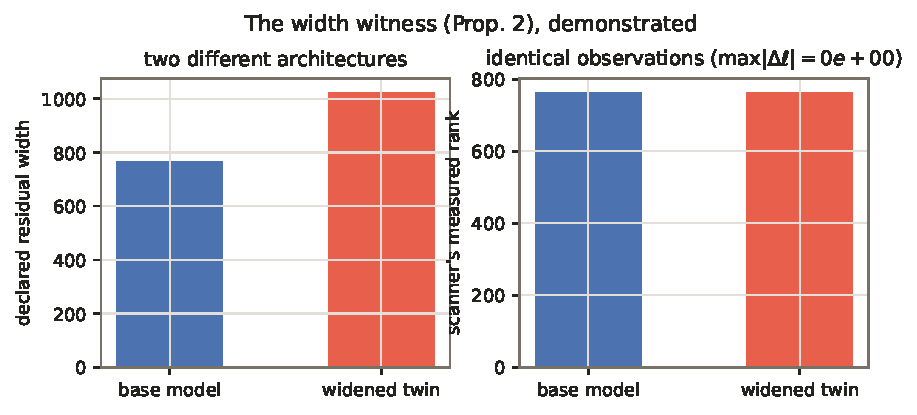
\includegraphics[width=.85\textwidth]{figures/fig_v4_witness.pdf}
\caption{Prop.~\ref{prop:rank} demonstrated.  A width-768 model and a constructively
widened width-1024 twin produce bit-identical logit outputs ($\max|\Delta\ell|=0$ over
\WitnessPrompts{} prompts $\times$ top-20), and the scanner's geometry probe measures the
same rank for both.  Width beyond the logit rank is structurally non-identifiable.}
\label{fig:witness}
\end{figure}

\subsection{The cost of separating what \emph{is} separable}
\label{sec:kappa}
Some properties are not blocked by a witness.  They are just expensive.  To price them
we use a single number per channel, $\kappa$, which we read as \emph{information per
request}.  It says how much useful evidence one API query gives us for telling two
competing hypotheses apart, measured in nats (the natural-log unit of information).  If
$\kappa$ is high, say around 2, then the decode-timing question is a strong question
for telling a transformer from an SSM: one or two requests settle it.  If $\kappa$ is
low, say around 0.02, each request moves the needle only slightly, and we need many of
them.  If $\kappa$ is exactly zero, no budget helps, because every allowed request
returns the same answer under both hypotheses.  The bound below turns $\kappa$ into a
minimum request count.

\begin{proposition}[Conditional query-cost lower bound]
\label{prop:cost}
Let two candidates have conditional observation laws $P_0^p,P_1^p$ for probe $p$, with
cost $c(p)>0$, and suppose every admissible conditional probe satisfies
$D_{\mathrm{KL}}(P_0^p\Vert P_1^p)\le\kappa\,c(p)$.  Then any adaptive test with type-I
and type-II errors at most $\delta<1/2$ needs
$\mathbb E_0[\mathrm{cost}]\ge(1-2\delta)\log\frac{1-\delta}{\delta}\,/\,\kappa$.
\end{proposition}
\begin{proof}
Apply the chain rule to the adaptive transcript (the policy itself adds no conditional
divergence), bound each probe by $\kappa$ times its cost, and pass the result through
the binary decision by data processing.  For random stopping, truncate and take limits.
\end{proof}
Here is what the bound says in everyday terms.  The numerator is the amount of evidence
a test needs to be wrong at most a fraction $\delta$ of the time.  At $\delta=0.05$ it
works out to about 2.65 nats.  Divide that by $\kappa$, the evidence per request, and
you get the smallest number of requests any strategy can get away with.  In version 2
of this manuscript the bound was stated without a value for $\kappa$: a shape without
numbers.  We now estimate $\kappa$ for each channel from benchmark and serving data
(Table~\ref{tab:kappa}).  Under the stated probe families, the fitted discrimination
models give a nominal lower-bound scale of about \KappaTokReq{} requests at
$\delta{=}0.05$ to separate two near tokenizer families, against about
\KappaTimingReq{} requests for the decode-state channel to separate attention from a
constant state.  Inside the domain of Prop.~\ref{prop:tok}, $\kappa=0$ exactly, so no
budget helps.  We treat $\hat\kappa$ as an empirical description of how much a channel
is worth, not as a proof that the KL bound holds for every admissible probe.  The
guarantee is exactly as conditional as that assumption.  In short, $\kappa$ tells us
how steep the boundary is.

\begin{table}[t]\centering\small
\caption{Measured per-channel information per request, $\hat\kappa$ (nats per
request, bootstrap 95\% CI), for the hardest pair of hypotheses each channel must
separate, together with the nominal lower-bound \emph{scale} on request count at
$\delta=0.05$.  The bound is conditional on the stated probe family: a point estimate of
$\kappa$ does not by itself prove the global KL domination the theorem assumes.  The
$\kappa=0$ row is proved, not estimated.}
\label{tab:kappa}
\begin{tabularx}{\textwidth}{@{}Y l l r@{}}
\toprule\textbf{Channel / hardest pair} & $\hat\kappa$ (nats/req) & CI & nominal $N$ scale ($\delta{=}.05$)\\
\midrule
Decode-state timing: full attention vs SSM (same hardware) & \KappaTiming & \KappaTimingCI & \KappaTimingReq\\
Tokenizer counts: cl100k vs o200k (realistic prompt mix) & \KappaTok & \KappaTokCI & \KappaTokReq\\
Wire grid: fp32 vs bf16-rounded logprobs & \KappaWire & \KappaWireCI & \KappaWireReq\\
o200k\_base vs o200k\_harmony, plain-text domain & $0$ (Prop.~\ref{prop:tok}) & - & $\infty$\\
\bottomrule\end{tabularx}
\end{table}

\paragraph{The four-way boundary taxonomy.}  Every component in the paper carries one
of four labels.  \textbf{I} means identified: measured at grade L1 to L3.  \textbf{C}
means cost-limited: $\hat\kappa$ has been estimated, so resolving the component is a
budget question with a computed price.  \textbf{A} means access-limited: the channel we
would need is not exposed on this interface, and the observability section
(Sec.~\ref{sec:observability}) measures what closing each channel costs.  \textbf{N}
means non-identifiable: a scoped witness exists, and no admissible request can help.
This taxonomy replaces the vague phrase ``future work'' with a map you can act on.

\section{\benchname: a blind ground-truth benchmark}
\label{sec:bench}
The core weakness of version 2 was simple: its production claims rested on detectors
that had never been checked against a known answer.  \benchname{} fixes that.  We
serve \emph{known} models behind the same anonymous contract the scanner faces in
production, freeze the protocol, run the scanner, and only then look at the labels.

\subsection{Subjects and axes}
We serve \BenchN{} subjects (Table~\ref{tab:subjects}).  The dense decoders run from
128 to 2{,}048 in residual width: Pythia, OPT, GPT-2, DistilGPT-2, SmolLM, Qwen2.5-0.5B,
and TinyLlama-1.1B.  There are two Mamba SSMs (130M and 370M), two MoE subjects (the
trained OLMoE-1B-7B, and a random-init Mixtral mechanics subject), a random-init
DeepSeek-V3-config MLA mechanics subject, four masked encoders from the BERT family, and
one encoder-decoder (T5-small).  Around this core we vary the \emph{serving}, not the
weights: the same checkpoint computed in fp32, bf16, and fp16; with its wire values
rounded to bf16; with int8 dynamic quantisation; behind an 8-way batching condition;
and a router fixture that alternates two checkpoints behind one model name.  The
random-init subjects exercise real code paths (MoE routing, MLA attention) even though
their weights are meaningless.  We label them mechanics subjects and disable the
behavioural probes for them.

\textbf{Effective sample size.}  The \BenchN{} subjects are \emph{not} \BenchN{}
independent architectures.  They span \BenchArchs{} distinct base checkpoints.  The
serving axis adds five GPT-2 variant configurations (four completed; fp16 omitted) plus a
two-checkpoint router.  Those variants exist to measure serving confounds, not to
inflate $n$.  All headline accuracies therefore carry cluster-bootstrapped intervals at
the base-checkpoint level (Table~\ref{tab:accuracy}, \BenchClusters{} clusters), and we
never quote the variant-inflated count as architectural coverage.  \BenchNScored{} of
\BenchN{} subjects completed the frozen protocol.  The fp16-on-CPU variant ran out of
time budget, because fp16 emulation on a CPU is several times slower than fp32 or bf16.
We report it as omitted rather than quietly dropping it.

\subsection{The anonymous contract}
Every subject answers the same OpenAI-compatible \texttt{/v1/chat/completions} endpoint.
It provides honest usage accounting, top-$k$ logprobs with $k\le20$, \texttt{logit\_bias},
SSE streaming with server-reported per-token times (in the style of Azure's
\texttt{latency\_checkpoint}), a stated context cap, and an explicit
\texttt{measurement\_columns} diagnostic that is used \emph{only} in the rich-access
regime.  Ground truth is recorded from the loaded config classes, never typed by hand.
The scanner sees no headers, no model strings, and no config hints.

\subsection{Blindness and freezing}
Three mechanisms keep the benchmark honest.  (i) The battery protocol, meaning the probe
set, the sample sizes, the spectral thresholds, and the decode-growth decision
thresholds, is frozen in code and hashed (\texttt{protocol \ProtocolHash}) before any
label is analysed.  (ii) The controlled-change study is run commit-reveal.  The harness
draws each episode's label in secret, writes only a SHA-256 commitment to disk before
scanning, and after the scan the reveal is verified against the commitment
(Sec.~\ref{sec:blindfixtures}).  (iii) Detectors that failed during development are
documented in the appendix together with their fixes.  One was a curvature gate that
fired without any effect-size check; another was a units error in the decode-growth
slope.  The benchmark reports the \emph{repaired} instrument, and the failure log is
part of the record.

\subsection{What the benchmark measures}
For each property we report three things on the support scores actually shown in this
paper: top-1 accuracy, the Brier score, and the expected calibration error (ECE).  Top-1
accuracy asks whether the highest-ranked candidate is right.  The Brier score is the
mean squared gap between the score and the truth, so lower is better and 0 is perfect.
ECE asks whether a score of 0.8 is right about 80\% of the time.  All three are reported
under two prior views (the reference prior and the evidence-only flat prior) and one
sensitivity check (the legacy independent-factor combination).  For each numeric target
we report rank-recovery coverage by width and the relative error on resolved estimates,
separately for rich and for production-realistic access.  For each serving axis we
report how the detectors respond to changes in dtype, batching, and routing.  The
baselines (Sec.~\ref{sec:baselines}) run on the same recordings.

\section{Detector validation: how far does reconstruction go?}
\label{sec:howfar}
Every number in this section comes from \benchname{} subjects whose ground truth was
recorded from the loaded configs.  Detectors and thresholds were frozen before any label
was analysed.  Table~\ref{tab:accuracy} is the paper's central empirical object.
Table~\ref{tab:matrix} is its one-look summary: for each observable channel, the
property it bears on, its identifiability class, its measured accuracy, and the main
thing that can fool it.

\begin{table}[!htb]\centering\footnotesize
\caption{The observability matrix: what each API channel can establish about the hidden
system, measured on \benchname{}.  \textbf{Class} is the boundary label of
Sec.~\ref{sec:ident}: \textbf{I} identified, \textbf{C} cost-limited ($\hat\kappa$
priced), \textbf{A} access-limited (channel absent or weak here), \textbf{N}
non-identifiable (witness).  Accuracy is top-1 against ground truth.}
\label{tab:matrix}
\begin{tabularx}{\textwidth}{@{}p{1.9cm} p{2.5cm} c p{2.2cm} p{2.6cm} Y@{}}
\toprule
\textbf{Channel} & \textbf{Property} & \textbf{Class} & \textbf{Accuracy} & \textbf{Coverage} & \textbf{Main confound}\\
\midrule
usage (accounting) & tokenizer count-family & I$+$N & 18/24 exact, 5 abstain & registry-dependent & merge-sharing variants (Prop.~\ref{prop:tok})\\
generation & AR-compatible generation contract & I & 25/25 & all subjects & a 1-token output cap can mimic it\\
streaming timing & transformer vs SSM & C & 8/8 decided & 19 eligible; 11 abstain$^{\mathsection}$ & serving overhead at short spans\\
logprob geometry & bottleneck width & I$^\dagger$/A & 15/15 core & rich: to 2{,}048; top-5: 0/25 & rank $\le$ observed columns (Prop.~\ref{prop:rank})\\
timing $+$ jitter & dense vs MoE & C & 88\% & 25 subjects & batching, cache, token mix\\
wire values & numeric grid & C & 80\% & 25 subjects & transport vs compute rounding\\
behaviour & objective signature (gen/mask) & A & 80\% & 25 subjects & post-training rewrites it\\
decision canaries & branch isolation & I$^{\ddagger}$ & 10/10 vs 0/10 & JEV; perm. $p{=}2{\times}10^{-4}$ & physical readout open\\
\bottomrule
\multicolumn{6}{@{}l@{}}{\footnotesize $^\dagger$with the rich column channel; standard top-5 production access is class A.~~$^\ddagger$this endpoint.}\\
\multicolumn{6}{@{}l@{}}{\footnotesize $^{\mathsection}$eligible = causal, non-router subjects: 8 decided $+$ 11 abstained $=$ 19.}\\
\multicolumn{6}{@{}l@{}}{\footnotesize ~~~n/a: 4 encoders, encoder-decoder, router; Table~\ref{tab:accuracy}'s $n{=}21$ adds recall on the last two.}
\end{tabularx}
\end{table}

\begin{table}[t]\centering\small
\caption{Reconstruction accuracy and calibration on \benchname{} (top-1 of the support
distribution against recorded ground truth).  Both the reference-prior and the
evidence-only (flat-prior) views are reported, because the difference between them is
itself informative (Sec.~\ref{sec:familysplit}).  $n$ varies: a property is scored only
where ground truth is defined (for example, KV sharing has no meaning for encoders or
SSMs).  Top-1 intervals are cluster-bootstrapped at the base-checkpoint level, so serving
variants of one checkpoint do not count as independent architectures (\BenchClusters{}
clusters).}
\label{tab:accuracy}
\begin{tabularx}{\textwidth}{@{}l c c c c c c Y@{}}
\toprule
\textbf{Property} & $n$ & \textbf{Top-1} & \textbf{95\% CI$^\dagger$} & \textbf{Top-1 (evid.-only)} & \textbf{Brier} & \textbf{ECE} & \textbf{Note}\\
\midrule
Core family & 24 & 88\% & [70,100] & 92\% & 0.300 & 0.169 & P23 split inside; prior lag on SSM analysed in Sec.~\ref{sec:familysplit} \\
FFN sparsity & 25 & 88\% & [71,100] & 88\% & 0.436 & 0.335 & weakest detector; production claims discounted \\
Serving topology & 25 & 96\% & [86,100] & 96\% & 0.284 & 0.360 & router fixture included \\
Wire precision & 25 & 80\% & [64,93] & 72\% & 0.221 & 0.169 & wire grid; int8 reads continuous by design \\
Attention/state regime & 21 & 90\% & [76,100] & 38\% & 0.460 & 0.477 & recall + decode-state, short spans \\
KV sharing & 6 & 67\% & [33,100] & 17\% & 0.507 & 0.067 & prior-only on production; bench measured where defined \\
Objective signature & 25 & 80\% & [60,95] & 96\% & 0.230 & 0.164 & causal vs masked vs prefix \\
\bottomrule
\multicolumn{8}{@{}l@{}}{\footnotesize $^\dagger$cluster bootstrap at the base-checkpoint level (serving variants of one checkpoint are one cluster).}\\
\end{tabularx}

\end{table}


\begin{figure}[t]\centering
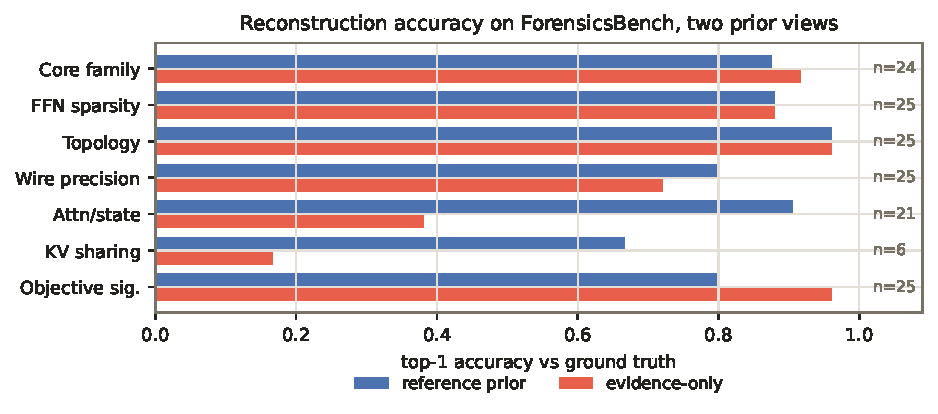
\includegraphics[width=.92\textwidth]{figures/fig_v4_accuracy.pdf}
\caption{Per-property top-1 accuracy under the reference prior (blue) and the
evidence-only flat prior (red).  The two views disagree exactly where a strong prior
meets a single decisive channel (core family, attention/state).}
\label{fig:accuracy}
\end{figure}

\subsection{The generation contract and the family split}
\label{sec:familysplit}
The generation test establishes what we call the \emph{autoregressive-compatible
generation contract}.  It looks at three things: how long a continuation the model
produces, whether latency grows with output length, and how finely the stream is
chunked.  This is deliberately a claim about the contract, not the architecture.  A
serving wrapper that returns at most one token per request could produce the same
observations with no autoregressive model behind it.  So the architecture-level reading
inherits that caveat, and the transformer-versus-SSM split below is what carries the
architecture-level discrimination.  Across \benchname{} the contract row is correct on
\FamilyPathAcc{} subjects, including both Mamba SSMs.  That is as it should be: SSMs
\emph{are} autoregressive at the contract level.  Our earlier draft featured a
``decoder-only 0.97'' score that silently blurred this distinction.  On the benchmark
that score is exactly as uninformative as a sceptical reviewer would expect, because
both SSM subjects score it too.

Telling a transformer from an SSM needs a different observable: the \emph{decode state}.
A transformer keeps a key-value cache that grows with every token, so each new token
costs slightly more time than the last.  An SSM keeps a state of fixed size, so the
per-token time stays flat.  The decode-state probe (P23) measures this slope from
streaming per-token times at contexts of 64 to 2048 tokens, which is inside every
deployment cap, taking the per-length minimum to suppress interference from other
tenants.  On \benchname{} the split is \SsmSplitAcc{} of the \SsmEligible{} eligible
subjects, meaning the causal, non-router ones.  The remaining six of 25 are structurally
ineligible: 4 encoders, the encoder-decoder, and the router (Fig.~\ref{fig:attncontrol}).
On the same-hardware control it separates full attention (+18.6\,\textmu s per token
per 1k of context, CI [16.3, 21.1]) from a 256-token sliding window (+1.8 [1.1, 2.6])
and from Mamba (+0.5 [$-0.0$, 1.2]).  We ran 60 trials per arm; only 3 were needed for
80\% power.  Two honest qualifications.  (i) Under the reference prior the categorical
call lags behind the evidence.  The prior odds against an SSM are 12 to 1, so a single
decisive channel moves SSM to top-1 only in the evidence-only view.  We show both.
(ii) On production endpoints with high serving overhead the channel is drowned in noise
at the spans we can reach, and there the probe abstains rather than guessing
(Sec.~\ref{sec:production}).

\begin{figure}[t]\centering
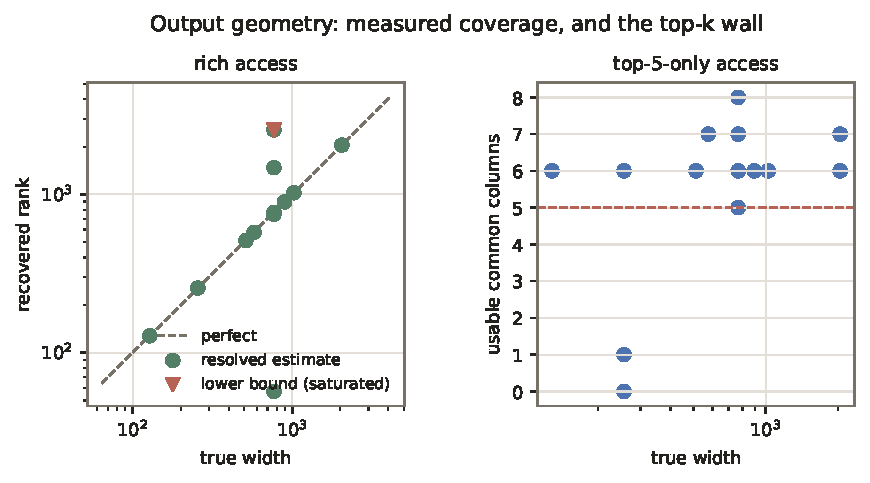
\includegraphics[width=\textwidth]{figures/fig_v4_geometry.pdf}
\caption{Left: recovered output-bottleneck rank against true width under rich access.
The adaptive ladder resolves widths up to 2{,}048 and reports lower bounds when it
saturates.  The visible off-diagonal cases are serving-axis artifacts, discussed in the
text: int8 quantisation deflates the measured rank (57 against a true 768), bf16 wire
rounding inflates it (2552 against 768), and the two-checkpoint router roughly doubles
it (1478).  The geometry channel detects the routing fixture that the topology prior
misses.  Right: under top-5-only access the usable common column set is a handful.  The
rank is capped by the observed columns (Prop.~\ref{prop:rank}), so width stays
unresolved.}
\label{fig:geometry}
\end{figure}

\subsection{Output geometry: coverage by width, and the top-\emph{k} wall}
\label{sec:geometry}
With the rich selected-column channel, the geometry protocol now \emph{adapts the
number of prompt rows to the width it is looking for}.  The ladder runs from 384 to
2560 rows, with a fixed relative threshold of $10^{-6}$ and a resolution gate fixed
before measurement.  The result is resolved estimates at widths \GeomResolvedList{},
which covers every core subject from 128 through 896, the 1{,}024-wide subject, and both
2{,}048-wide subjects, with relative errors under \GeomMaxErr{}, and lower bounds beyond
that.  At width 2{,}048 the ladder saturates at its 2{,}560-row cap and yields a lower
bound rather than a point estimate.  We report the bound.  Under the
production-realistic top-5-only regime, \emph{no} subject resolves.  The natural top-5
column union spans only \TopFiveCols{} columns on average, so the matrix rank is capped
by construction.  That is Prop.~\ref{prop:rank} made empirical.  This is the honest shape
of the claim: \textbf{width recovery is a budgeted capability that depends on the access
regime and comes with a measured coverage curve.  It is not a demo.}

\subsection{Numeric regime, tokenization, sparsity}
The wire-grid detector scores \DtypeAcc{} across the dtype variants (fp32, bf16, and
fp16 compute, plus the bf16-rounded wire).  The int8-dynamic case reads as a continuous
grid.  That is correct at the wire layer, and it is a documented limit on inferring the
compute dtype.  Tokenizer count-family matching is \TokenizerAcc{} exact within the
reference registry.  The domain-timing MoE detector is the weakest instrument, at
\MoeAcc{} top-1: small dense models served on CPU produce MoE-like timing signatures
often enough to matter.  We therefore report MoE on production \emph{at that measured
reliability}, and the interleaved-control follow-up (Sec.~\ref{sec:production}) replaces
the domain-timing signal where it matters.  The \emph{objective signature} row of
Table~\ref{tab:accuracy} measures the observable generation or masking contract (causal
versus masked versus prefix behaviour), not the historical training recipe.
Post-training can rewrite behaviour without touching the weights, so this row is named
and graded as a signature, never as a recovered training objective.

\paragraph{The prior/evidence gap is a measurement.}
The attention/state property scores \AttnRefAcc{} under the reference prior but only
\AttnFlatAcc{} under the evidence-only flat prior.  That is the largest prior-dependence
anywhere in the benchmark.  It is not merely a caveat.  It is a result about forensic
inference under weak channels: where the observable channel is thin (short-span recall
plus a noise-limited decode slope), confidence in an architectural property is driven
mostly by the structural prior.  The honest report is the pair of numbers, not either one
alone.  We report both views for every property precisely so that prior-driven support
is visible as such (Table~\ref{tab:accuracy}).

\begin{figure}[t]\centering
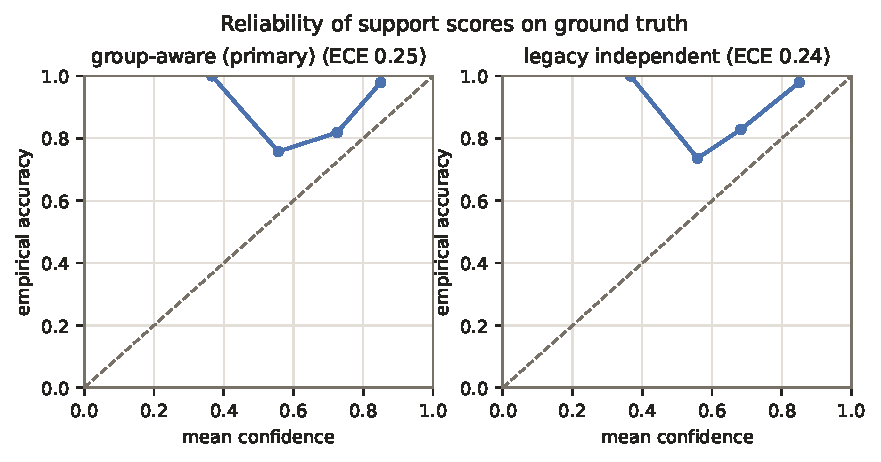
\includegraphics[width=.9\textwidth]{figures/fig_v4_reliability.pdf}
\caption{Reliability of support scores against \benchname{} ground truth: group-aware
ranker (left) versus the legacy independent-factor ranker (right).}
\label{fig:reliability}
\end{figure}

\subsection{Calibration: are the support scores honest?}
\label{sec:calibration}
Table~\ref{tab:calibration} reports the Brier score and ECE of the scores shown in this
paper, computed on \benchname{} labels, for the group-aware ranker (primary) and the
legacy independent-factor ranker (sensitivity).  The seven properties differ in how
many classes they have, how balanced those classes are, and how hard they are, so a
single pooled number would mix unlike prediction problems.  We therefore report the
\emph{macro-average} over properties with a property-bootstrap CI (ECE \BenchECE{}
\BenchECEMacroCI{}, Brier \BenchBrier{} \BenchBrierMacroCI{}) and the per-property values
in Table~\ref{tab:accuracy}.  Grouping protects against mechanically compounding
repeated evidence, which is the failure mode that motivated it.  But it does \emph{not}
improve these aggregate calibration metrics here (legacy: ECE \BenchECELegacy{}
\BenchECEMacroLegacyCI{}, Brier \BenchBrierLegacy{} \BenchBrierMacroLegacyCI{}).  We
report both schemes and claim no calibration improvement.  Scores remain support ranks,
never probabilities, and their rank order now carries a measured error rate per
property (Table~\ref{tab:accuracy}).

\begin{table}[h]\centering\small
\caption{Calibration of the support scores on \benchname{} ground truth,
macro-averaged over the seven heterogeneous properties of Table~\ref{tab:accuracy}
(each weighted equally, since their class counts and difficulties differ; CIs by
bootstrap over properties).  Per-property values appear in Table~\ref{tab:accuracy}.}
\label{tab:calibration}
\begin{tabular}{@{}l c c c c@{}}
\toprule
\textbf{Ranker} & \textbf{Brier} & 95\% CI & \textbf{ECE} & 95\% CI\\
\midrule
group-aware (primary) & 0.348 & [0.272,0.429] & 0.249 & [0.153,0.351] \\
legacy independent factors & 0.344 & [0.269,0.423] & 0.244 & [0.153,0.346] \\
\bottomrule
\multicolumn{5}{@{}l@{}}{\footnotesize Macro-averaged over the seven properties of Table~\ref{tab:accuracy} (equal weights);}\\
\multicolumn{5}{@{}l@{}}{\footnotesize CI by bootstrap over properties; per-property values in Table~\ref{tab:accuracy}.}\\
\end{tabular}

\end{table}

\section{Experimental-design validation}
\label{sec:design}
Having validated the detectors, we now validate the \emph{design} machinery around
them: the planner that chooses experiments, the published baselines run on the same
subjects, and the blind change-detection suite.

\subsection{Baselines on the same subjects}
\label{sec:baselines}
Different methods solve different problems under different observation regimes.  So we
compare \emph{on the same subjects, the same recordings, and the same access}, and we
report each method against its own target rather than forcing a single leaderboard
number.  NightVision-lite estimates width from the rank of the top-5 column union and
depth from inverted timing, holding hardware constant with a leave-one-out scheme.  It
resolves \NVWidthResolved{} widths, because its access regime cannot get past the top-5
wall either, and its depth estimates carry a median relative error of \NVDepthErr{} on
the subset where that estimator is defined.  LLMmap-lite fingerprinting identifies
\LLMmapIdent{} of subjects by nearest neighbour and classifies family at \LLMmapFam{}
(leave-one-out).  Neither baseline is a strawman.  Fingerprinting is the right tool for
the question \emph{which known model is this}, but it has no mechanism for an
architecture outside its reference set, which is what the router and mechanics subjects
are.  NightVision-style estimation targets weight-level dimensions that we deliberately
treat as access-limited here.  Our pipeline reports structure with measured reliability
and abstains where the channel is empty.  Head-to-head numbers on the shared subset are
in Table~\ref{tab:baselines}.

\begin{table}[h]\centering\small
\caption{Baselines on the same \benchname{} subjects, recordings, and access regime.
This is an apples-to-apples comparison on the shared subset, not a claim that one method
dominates another: fingerprinting identifies known models, NV-lite estimates dimensions
under top-5 access, and this paper reports partial identification with abstention.}
\label{tab:baselines}
\begin{tabularx}{\textwidth}{@{}Y Y Y@{}}
\toprule
\textbf{Method} & \textbf{Geometry} & \textbf{Identity/family}\\
\midrule
NightVision-lite (top-5 width + timing depth) & 0/2 widths & median depth err 30\% (n=3$^*$) \\
LLMmap-lite (24-prompt fingerprint) & identification 71\% & family 35\% (n=26) \\
\textbf{This paper} & geometry resolved 15/15; family 88\% & graded support, abstention with named next step \\
\bottomrule
\multicolumn{3}{@{}l@{}}{\footnotesize Same subjects, same recordings, same access regime. $^*$NV-lite's timing-inverted depth is defined only where its precondition holds.}\\
\end{tabularx}

\end{table}

\subsection{The planner, live}
\label{sec:plannerlive}
We re-ran the planner comparison \emph{live}, with no replay of saved logs:
\PlannerSeeds{} seeds per subject per planner against the simulator, with per-seed
serving jitter, request budgets, and a frozen recovery target.  The honest headline is
mixed, and we report it as measured.  On requests-to-top-1 all three planners tie,
because the baseline sweep already suffices on easy subjects.  On
requests-to-\emph{decisive-discriminator evidence}, meaning how many requests it takes
before the one probe that actually settles the family question has run, the simple
cheapest-first static ordering is \emph{not} beaten by the information-gain planner.
Static lands the discriminator at \PlannerStaticDecisive{} requests, against
\PlannerEigDecisive{} for EIG and \PlannerUniformDecisive{} for uniform ordering on the
family-split subjects.  The reason is mundane: the cheap probes happen to include the
discriminators.  The pathologies are the real findings.  (i) A pure EIG surrogate starves
the very probe that could unseat a confident front-runner, because the surrogate assigns
the upset a low probability and so expects little gain from it.  The engine now carries a
\emph{core-coverage floor}: before the diminishing-returns stop fires, at least one
high-diagnosticity challenger must have run for every core property.  Without that floor,
EIG never runs the decisive probe on the SSM subject at all.  (ii) Under the strong
reference prior, the SSM target stays uncrossed within budget for every planner.
Planning cannot beat a prior; only evidence can (Sec.~\ref{sec:familysplit}).
Table~\ref{tab:planner} has the full matrix, and Fig.~\ref{fig:planner} shows the
per-subject picture.

\begin{figure}[t]\centering
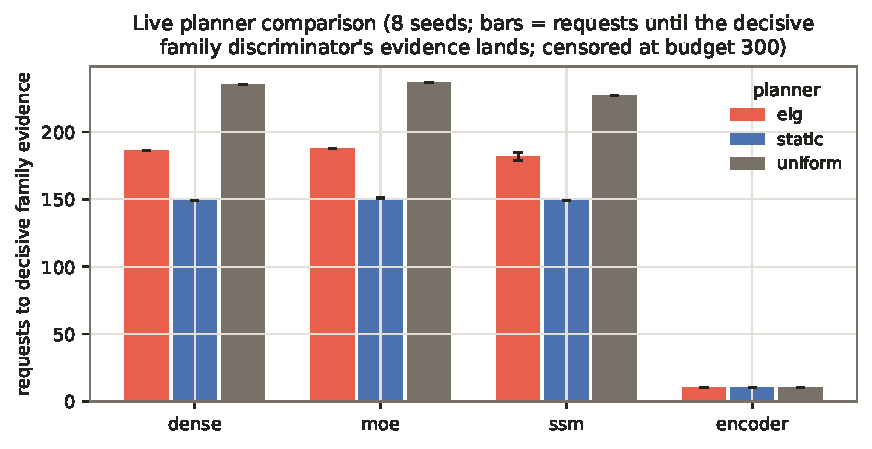
\includegraphics[width=.92\textwidth]{figures/fig_v4_planner.pdf}
\caption{Live planner comparison (8 seeds, per-seed serving jitter).  Requests until
the decisive family discriminator's evidence lands.}
\label{fig:planner}
\end{figure}

\begin{table}[h]\centering\small
\caption{Live planner comparison (no replay): requests to the top-1 family target and to
arrival of decisive family evidence (P23/P19-prefill), mean [95\% CI] over 8 seeds,
$\dagger$ = censored at the 300-request budget.}
\label{tab:planner}
\begin{tabular}{@{}l l c c c@{}}
\toprule
\textbf{Subject} & \textbf{Planner} & \textbf{req $\to$ top-1} & \textbf{req $\to$ decisive} & \textbf{censored}\\
\midrule
dense & eig & 8 [8,8] & 186 [186,186] & 0\% \\
dense & static & 8 [8,8] & 149 [149,149] & 0\% \\
dense & uniform & 8 [8,8] & 235 [235,235] & 0\% \\
encoder & eig & 10 [10,10] & 10 [10,10] & 0\% \\
encoder & static & 10 [10,10] & 10 [10,10] & 0\% \\
encoder & uniform & 10 [10,10] & 10 [10,10] & 0\% \\
moe & eig & 8 [8,8] & 188 [188,188] & 0\% \\
moe & static & 8 [8,8] & 151 [151,151] & 0\% \\
moe & uniform & 8 [8,8] & 237 [237,237] & 0\% \\
ssm & eig & 300 [300,300] & 182 [179,185] & 0\% \\
ssm & static & 300 [300,300] & 149 [149,149] & 0\% \\
ssm & uniform & 300 [300,300] & 227 [227,227] & 0\% \\
\bottomrule
\end{tabular}

\end{table}

\begin{figure}[t]\centering
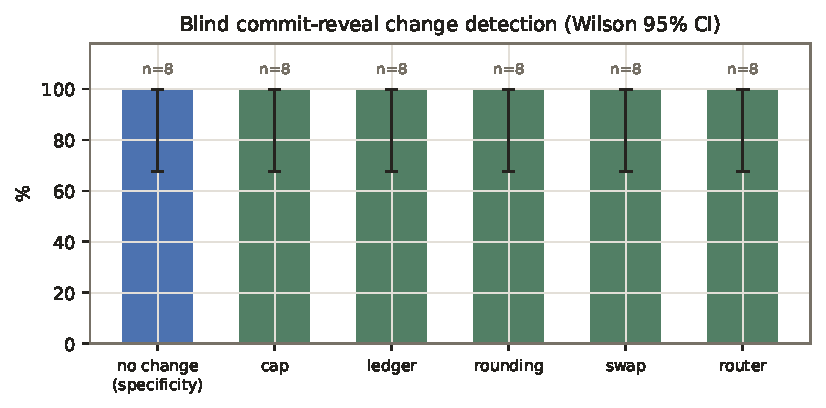
\includegraphics[width=.8\textwidth]{figures/fig_v4_blind.pdf}
\caption{Blind commit-reveal change detection (Wilson 95\% CIs).}
\label{fig:blind}
\end{figure}

\subsection{Blind controlled changes}
\label{sec:blindfixtures}
The fixture suite is now a blind test.  The harness draws each episode's label and
commits it as a SHA-256 hash before the scan.  The detectors are frozen.  After the
scan, the reveal is checked against the commitment.  Over \BlindN{} episodes the
sensitivities are: cap change \BlindCap{}, ledger inflation \BlindLedger{}, wire
rounding \BlindRound{}, checkpoint swap \BlindSwap{}, and router alternation
\BlindRouter{}, with \BlindNone{} specificity on unchanged controls (Wilson 95\% CIs in
Table~\ref{tab:blind}).  These are \emph{large, designed} changes.  The suite measures
the detection floor, not the rate of wrong claims on a real population.

\begin{table}[h]\centering\small
\caption{Blind commit-reveal fixture results (detectors frozen; labels committed by hash
before each scan).}
\label{tab:blind}
\begin{tabular}{@{}l c c c@{}}
\toprule
\textbf{Episode} & \textbf{Rate} & \textbf{Wilson 95\% CI} & $n$\\
\midrule
no change (specificity) & 100\% & [68,100]\% & 8 \\
output-cap change & 100\% & [68,100]\% & 8 \\
ledger inflation & 100\% & [68,100]\% & 8 \\
wire rounding & 100\% & [68,100]\% & 8 \\
checkpoint swap & 100\% & [68,100]\% & 8 \\
router alternation & 100\% & [68,100]\% & 8 \\
\bottomrule
\end{tabular}

\end{table}

\begin{figure}[t]\centering
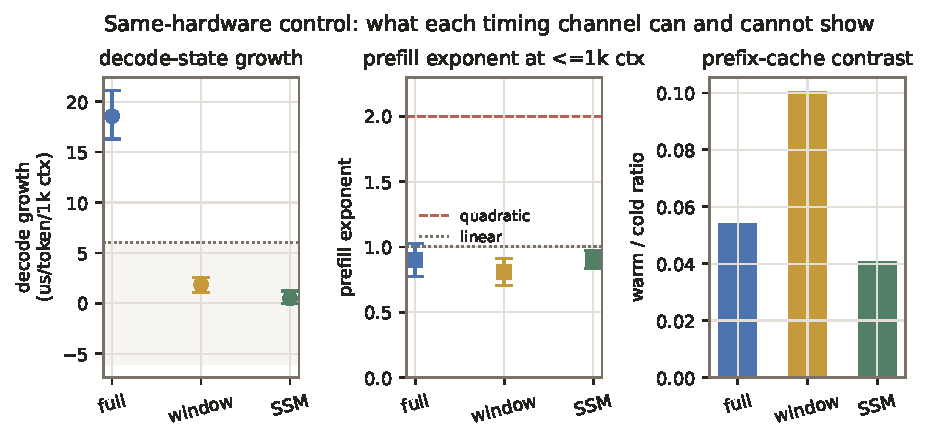
\includegraphics[width=\textwidth]{figures/fig_v4_attncontrol.pdf}
\caption{Same-hardware control (GPT-2 full attention; Mistral-config 256-token sliding
window; Mamba-config constant state; 60 trials per arm, $\ge$3 needed for 80\% power).
\textbf{Left:} decode-state growth separates the three mechanisms cleanly.
\textbf{Middle:} fresh-prefill exponents at $\le$1k context are sub-quadratic for
\emph{all} mechanisms, so prefill curvature tells you nothing at short span.
\textbf{Right:} the prefix-cache contrast (warm/cold 0.04--0.10) is the effect that
contaminated naive fresh-versus-repeat comparisons.}
\label{fig:attncontrol}
\end{figure}

\subsection{Same-hardware attention control}
\label{sec:attncontrol}
Figure~\ref{fig:attncontrol} is the control that the production DSA interpretation
needed.  We served three stacks on identical hardware: full attention (GPT-2), a
sliding window of 256 tokens (Mistral-config), and a constant state (Mamba-config), and
measured all three with the production protocol.  Decode growth separates the
mechanisms decisively.  Fresh-prefix prefill exponents at $\le$1k context are all
between $0.8$ and $0.9$, which is sub-quadratic for \emph{every} mechanism at that span.
That is why any claim based on prefill curvature needs long context.  The warm-versus-cold
prefix contrast is a factor of 5 to 10, which shows how large the cache effect is that
contaminated naive fresh-versus-repeat comparisons.  Every production timing claim in
Sec.~\ref{sec:production} is graded against this control.

\section{Production reconstructions, graded by measured reliability}
\label{sec:production}
We now return to the three production endpoints.  They are \emph{demonstrations} of the
measured instrument, not the contribution itself.  Every component below carries three
things: (i) its evidence grade, (ii) the probe that produced it, and (iii) that probe's
measured reliability on \benchname{} from Sec.~\ref{sec:howfar}.  One caveat applies to
everything in this section.  The reliabilities were measured on \benchname{} under its
own observability and serving regime.  Carrying those error rates over to a frontier
production deployment is an assumption about external validity, because the benchmark
and production are different populations: CPU serving against accelerated serving, and
known checkpoints against frontier stacks.  In symbols, $P_{\rm production}\neq P_{\rm
benchmark}$.

\begin{figure}[t]\centering
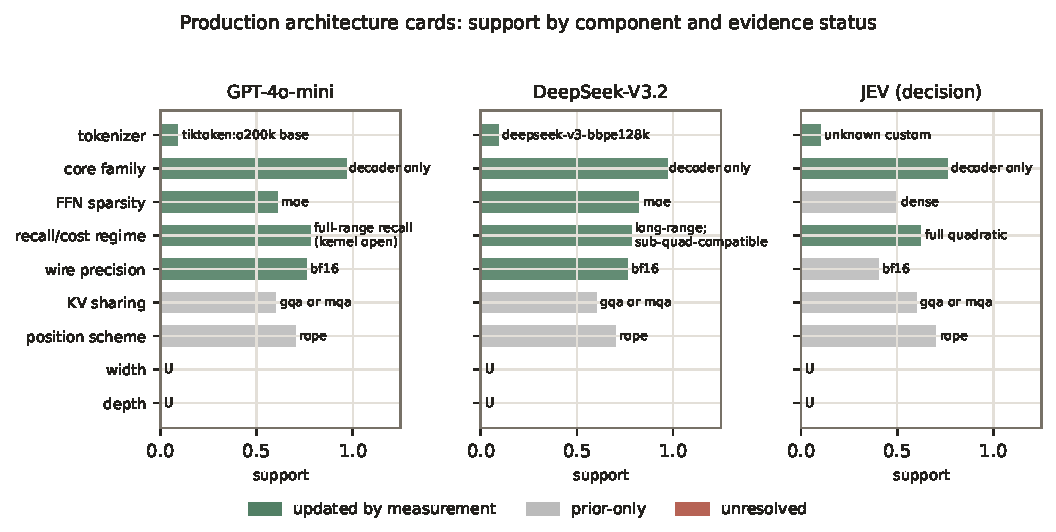
\includegraphics[width=\textwidth]{figures/fig_v4_cards.pdf}
\caption{Production architecture cards: per-component support with evidence status
(green = updated by measurement, grey = prior-only, red/U = unresolved).  Generated from
the recorded scan posteriors; the attention row carries the powered follow-up's reading,
not the recall-only prior.}
\label{fig:cards}
\end{figure}

\subsection{GPT-4o-mini: the worked reconstruction}
\label{sec:gptcase}
The eight-step progression (Fig.~\ref{fig:recongpt}) shows the instrument at work on an
opaque endpoint.  Each step says what it can establish and what it cannot.
\begin{enumerate}[nosep,leftmargin=1.6em,label=\textbf{\arabic*.}]
\item \textbf{Interface boundary.} An over-limit request reads the deployment contract
  straight from the error text: 16{,}384 maximum completion, 16{,}393-token accepted
  input (L1).  The model's documented capability is larger \cite{openaimini2024docs}.
  This is a fact about the interface layer, not the model (Sec.~\ref{sec:layers}).
\item \textbf{Tokenization.} Count differences on a fixed scaffold match
  \texttt{o200k\_base} and \texttt{o200k\_harmony} on all 18 strings.  That is a
  count-family identification with a proved tie (Prop.~\ref{prop:tok}), L2.
\item \textbf{Generation path.} A 24-token continuation whose latency rises with output
  length (23\,$\to$\,202\,ms) establishes the autoregressive-compatible generation
  contract, L2.  This is contract-level, not transformer-specific
  (Sec.~\ref{sec:familysplit}).
\item \textbf{Attention/state regime.} 18 of 18 needle retrievals succeed through 8{,}225
  tokens, which establishes full-range recall.  The attention kernel itself stays
  unseparated at these spans (L4; Fig.~\ref{fig:attncontrol}).
\item \textbf{KV sharing / positions.} GQA/MQA and RoPE appear only as priors.  They
  are shown in grey and never counted as recovered.  The discriminators that would decide
  them are recorded by name.
\item \textbf{Numeric regime.} The logprob lattice is consistent with bf16 (support 0.76),
  L4 at the wire layer.
\item \textbf{Feed-forward.} Dense or MoE is ambiguous (0.61 against 0.39).  It is reported
  at the detector's measured \MoeAcc{} reliability, with the interleaved control
  returning a null.
\item \textbf{Width/depth.} Width is unresolved by access (the top-5 wall,
  Prop.~\ref{prop:rank}).  Depth is unresolved by confound (compute and queueing are
  tangled).  Both are U with named next experiments.
\end{enumerate}

\begin{figure}[t]\centering
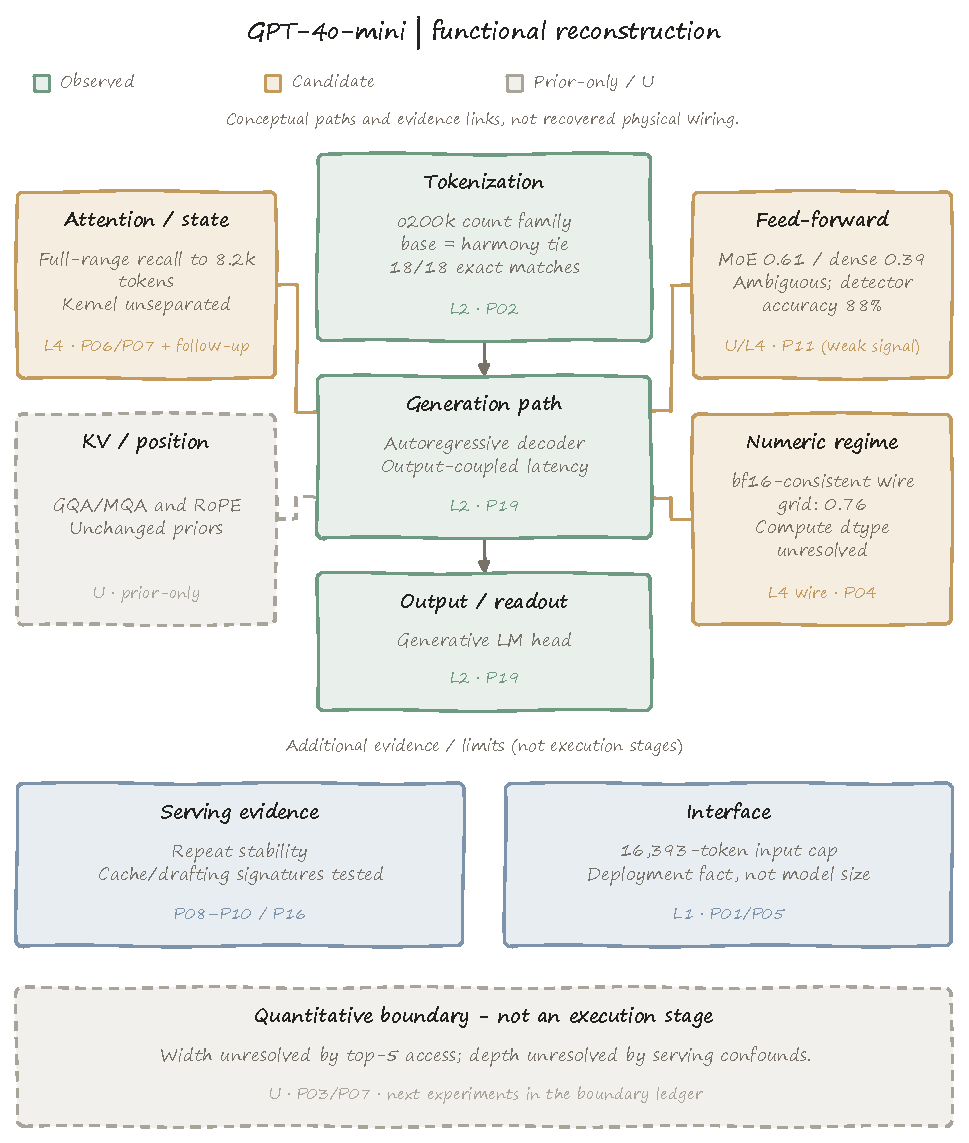
\includegraphics[width=\textwidth]{figures/fig_v4_recon_gpt.pdf}
\caption{GPT-4o-mini functional reconstruction.  Cards distinguish observed properties,
mechanism candidates, unchanged priors, and unresolved components.  Arrows show
conceptual functional order; side links associate evidence with a component, not
measured physical wiring.  The quantitative boundary is separate from the path.}
\label{fig:recongpt}
\end{figure}

\begin{table}[h]\centering\small
\caption{GPT-4o-mini: reconstructed components.  ``Bench'' is the detector's measured
accuracy on \benchname{}; grey rows are prior-only (no updating evidence).}
\label{tab:gptcard}
\begin{tabularx}{\textwidth}{@{}l Y c l Y@{}}
\toprule
\textbf{Component} & \textbf{Reconstruction} & \textbf{Grade} & \textbf{Bench} & \textbf{Basis}\\
\midrule
Input/output boundary & 16{,}393-token deployment cap; 16{,}384 max completion & L1 & - & error text; docs note larger model capability\\
Tokenizer & o200k count family (base$=$harmony tie) & L2 & 18/24 exact & 18/18 fixed-scaffold count matches (Prop.~\ref{prop:tok} tie)\\
Generation path & AR-compatible contract & L2 & 25/25 & 24-token continuation; latency scales with output\\
Transformer vs SSM & transformer-consistent, short span & U & 8/8 decided & engine decode TBT 11\,ms flat, CI $[-74,+86]$\,\textmu s/tok/1k (noise-dominated)\\
Attention regime & full-range recall to 8{,}225 tokens & L4 & - & 18/18 needle conditions; prefill exponent \GptFreshExp{} \GptFreshCI{} at $\le$15k\\
Wire numerics & bf16-consistent lattice & L4 & 80\% & P04 grid match\\
Feed-forward & dense/MoE ambiguous (MoE 0.61) & U & 88\% & domain timing weakest; interleaved control null\\
KV / position & GQA/MQA, RoPE (priors only) & U & - & no updating evidence; named next experiments\\
Width / depth & unresolved & U & - & top-5 access wall (Prop.~\ref{prop:rank}); compute$\times$queueing confound\\
\bottomrule
\end{tabularx}
\end{table}

\begin{figure}[t]\centering
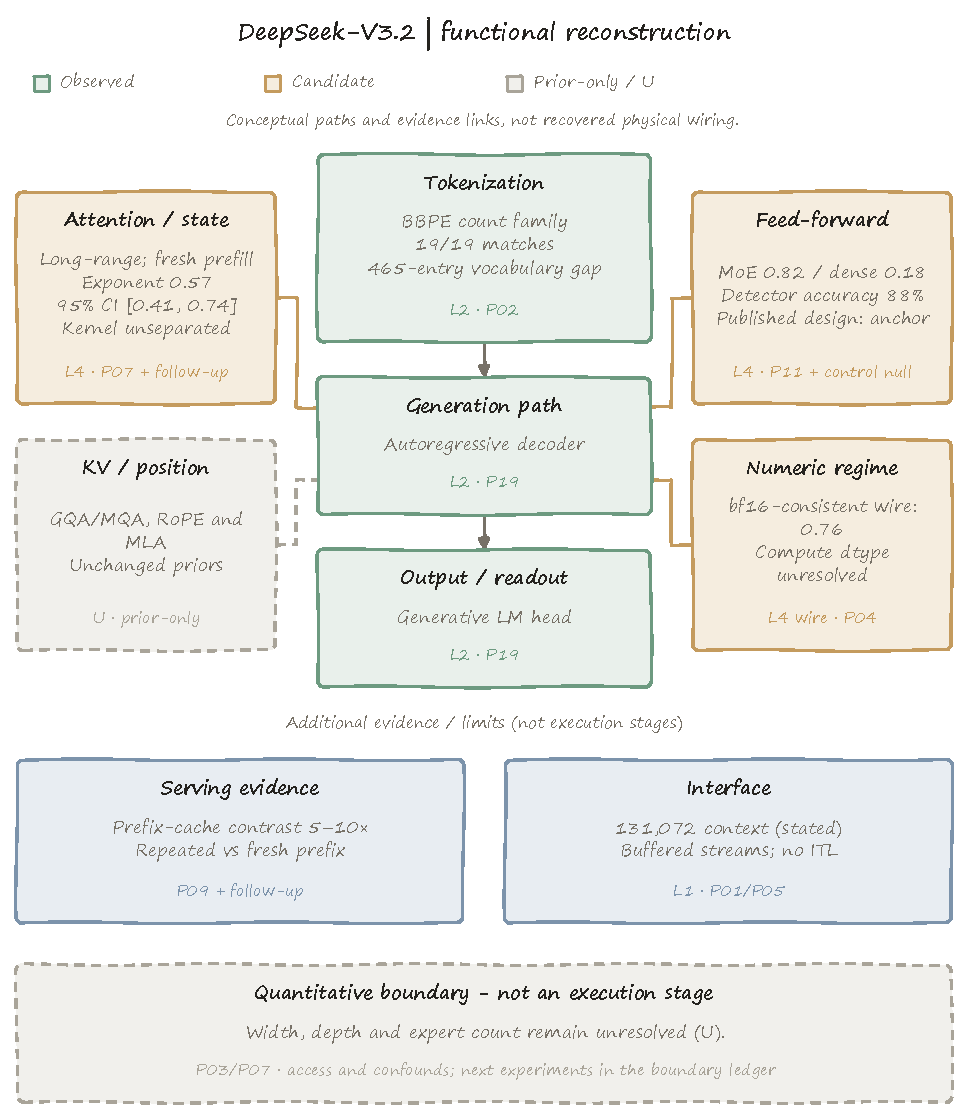
\includegraphics[width=\textwidth]{figures/fig_v4_recon_deepseek.pdf}
\caption{DeepSeek-V3.2 functional reconstruction: MoE-leaning feed-forward and
long-context evidence with unresolved alternatives.  Side links are evidence
associations, not physical wiring; the published design is an evaluation anchor,
not a measurement.  Width, depth, and expert count remain unresolved.}
\label{fig:recondeep}
\end{figure}

\subsection{DeepSeek-V3.2}
The same battery reconstructs a BBPE count-family tokenizer (19 of 19 matches), an
autoregressive decoder path, and a stated 131{,}072-token context.  Two claims carry
the paper's production weight.

\paragraph{MoE-leaning feed-forward.}  The domain and jitter signatures give MoE 0.82
against dense 0.18, and the published design is indeed MoE.  But our own benchmark says
this class of detector is only \MoeAcc{} accurate.  So we report the lean \emph{and} the
discount together.  The interleaved, length-matched, one-token control (10 randomised
blocks with domain-label permutation) does not reject the null of no domain effect on
either endpoint, which weakens the timing discriminator.  The jitter signature remains.
Grade: L4, mechanism-consistent with an independent published anchor.  Not L2.

\begin{figure}[t]\centering
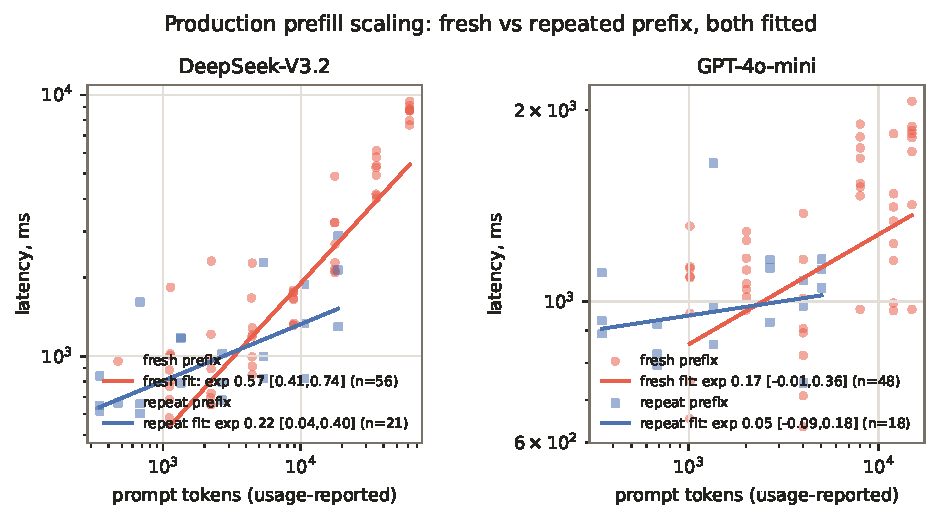
\includegraphics[width=\textwidth]{figures/fig_v4_prodscaling.pdf}
\caption{Production prefill scaling, powered follow-up: fresh-nonce (red) against
repeated-prefix (blue), both fitted with the same log-log model.  DeepSeek's fresh
exponent is sub-quadratic (\DsFreshExp{}, CI \DsFreshCI{}, $n$=\DsFreshN{});
GPT-4o-mini's prefill is overhead-dominated at these spans (\GptFreshExp{}, CI
\GptFreshCI{}, $n$=48).  Exponents constrain the attention node; they do not uniquely
select a kernel (Fig.~\ref{fig:attncontrol}).}
\label{fig:prodscaling}
\end{figure}

\paragraph{Fresh-prefix prefill scaling.}  The v2 comparison mixed a fitted
repeated-prefix curve with eight unfitted fresh-nonce points.  Most of what it showed
was a prefix-cache artifact.  The powered follow-up (Fig.~\ref{fig:prodscaling}) fits
both curves with the same log-log model on randomised trials.  A log-log fit means we
plot the logarithm of time against the logarithm of context length; the slope of that
line is the scaling exponent, where 1 means linear and 2 means quadratic.  The fresh
exponent is \DsFreshExp{} (95\% CI \DsFreshCI{}, $n=\DsFreshN$); the repeated-prefix
exponent is \DsRepeatExp{} (\DsRepeatCI{}, $n=\DsRepeatN$).  The fresh curve is
sub-quadratic, which is compatible with the documented sparse attention
\cite{deepseekai2025v32}.  But our same-hardware control (Fig.~\ref{fig:attncontrol})
shows that small dense models at short spans also look sub-quadratic.  So the exponent
does not \emph{select} DSA.  It narrows the attention node to candidates that are
compatible with sub-quadratic scaling.  Grade: L4, not L2.

\begin{figure}[t]\centering
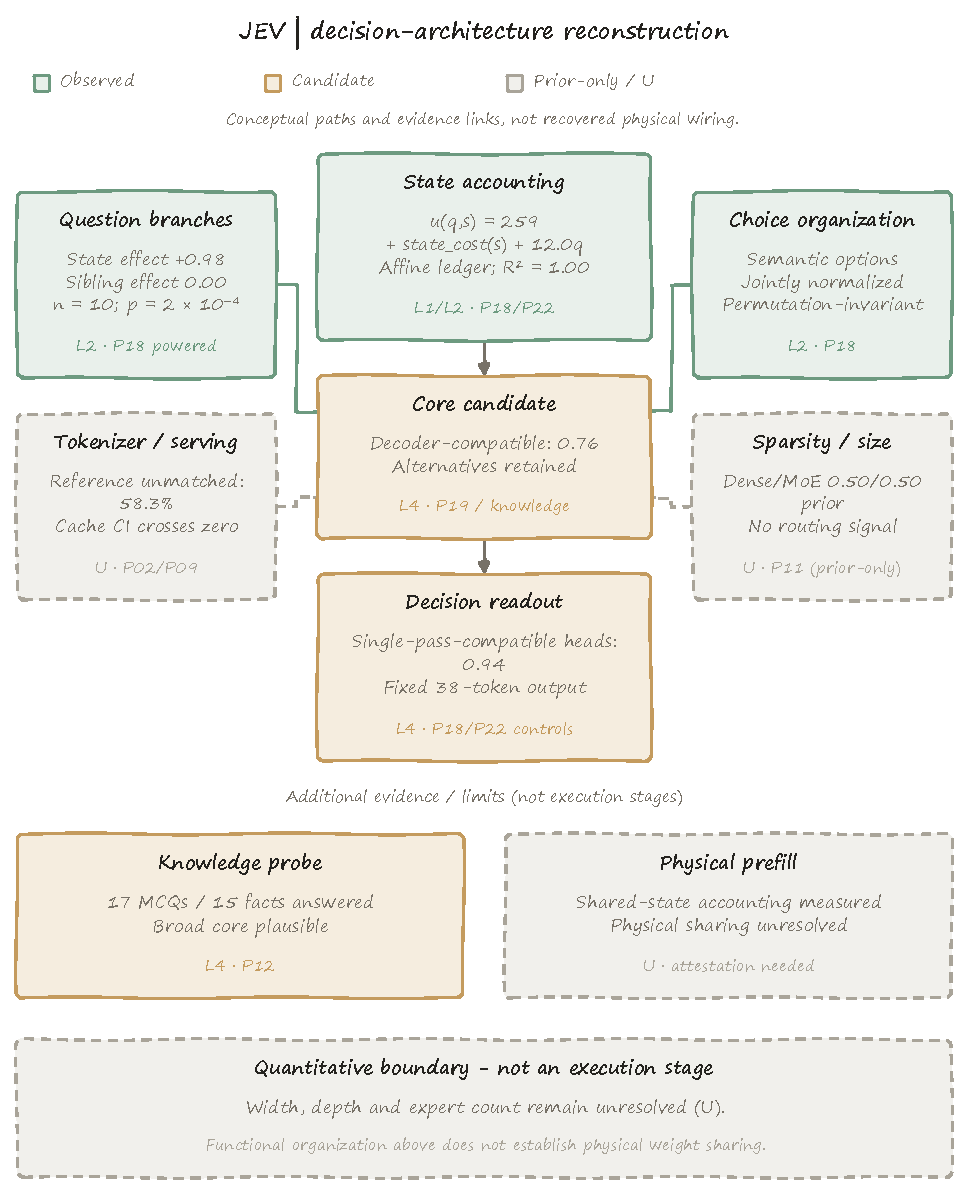
\includegraphics[width=\textwidth]{figures/fig_v4_recon_jev.pdf}
\caption{JEV's decision reconstruction: measured state accounting, isolated branches,
and normalized choices alongside a candidate core and single-pass-compatible readout.
Side links associate evidence; neither these links nor the affine ledger establish
physical weight sharing.  The quantitative boundary remains unresolved.}
\label{fig:reconjev}
\end{figure}

\subsection{JEV: a cross-contract generality test, powered}
JEV plays one specific role in this paper.  It is the \emph{cross-contract generality
test}: proof that the instrument is not a trick that only works on text-generation
APIs, but also works on a decision endpoint with a different interface contract.  Its
reconstruction is unchanged in kind and stronger in evidence.  The shared-state
accounting follows an exact linear ledger, $u(q,s)=259+\mathrm{state\_cost}(s)+12.0q$
with $R^2=1.00$: a fixed 259 tokens, plus the cost of the state, plus 12 tokens per
question.  The branches are isolated, the semantic choices are normalized, and the
readout is a fixed 38 tokens.  In v2 the branch-isolation claim rested on three trials.
The powered follow-up runs $n=\JevSecrets{}$ fresh secrets $\times$ \{baseline,
secret-in-state, secret-in-sibling\} in randomised order.  Planting the secret in the
shared state moves the answer by +\JevStateEff{}; planting it in a sibling question
moves it by \JevSibEff{}; the permutation test gives $p=\JevPermP$
(Fig.~\ref{fig:jevpower}).  Isolated branches over a shared state are now an L2-grade
measured property of this endpoint, not a three-trial hint.

\begin{figure}[t]\centering
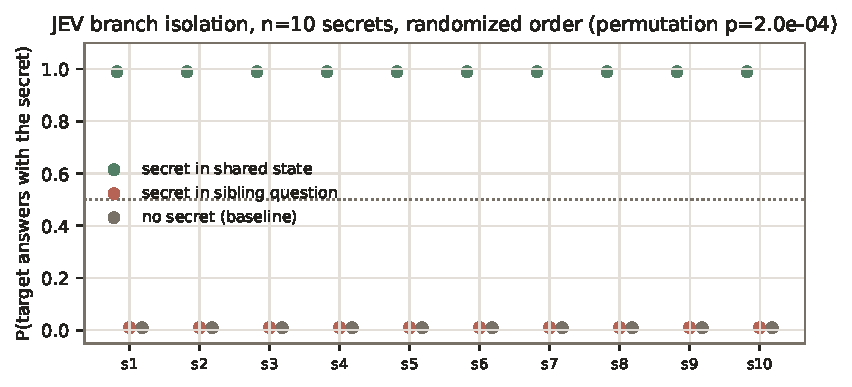
\includegraphics[width=.8\textwidth]{figures/fig_v4_jevpower.pdf}
\caption{JEV branch isolation, powered: $n$=10 fresh secrets, randomised order.  Secrets
in the shared state are used (+0.98); secrets in sibling questions are invisible (0/10,
permutation $p=2\times10^{-4}$).}
\label{fig:jevpower}
\end{figure}

\section{API observability: how the surface bounds the boundary}
\label{sec:observability}
The boundary is not fixed by nature.  It is set by what the provider chooses to expose.
This section measures that directly: how the identified set changes as channels are
closed one by one.

\subsection{Channel-closure ablation}
We take one synthetic stack and keep the model fixed while closing surfaces in
sequence: full access $\to$ a top-5 cap $\to$ logits closed $\to$ billing also closed
$\to$ added timing noise.  Table~\ref{tab:closure} shows how the detectors respond.
Closing the logits weakens the wire-grid and repeat evidence (the dtype score drops from
0.76 to 0.40).  Closing billing removes tokenizer acquisition entirely, because the
count channel is gone.  Closing both leaves the behavioural core intact (generation
family, contract) but stops every numeric reconstruction.  Adding timing noise at the
tested level changed nothing further.  This is a detector-response ablation on a single
stack.  It maps the \emph{direction} of each dependency.  It is not a universal proof
that closing a channel hides a property from every possible estimator.

\begin{table}[t]\centering\small
\caption{Same-model channel closure: settled-property count and key detector scores as
surfaces close.  ``--'' = channel absent, property unmeasurable.}
\label{tab:closure}
\begin{tabularx}{\textwidth}{@{}l r r r X@{}}
\toprule
\textbf{Surface} & \textbf{Scores $\geq .65$} & \textbf{Wire dtype score} & \textbf{Cache score} & \textbf{Tokenizer estimate} \\
\midrule
full & 17 & 0.76 & 0.86 & available \\
cap5 & 17 & 0.73 & 0.86 & available \\
-logit & 15 & 0.40 & 0.86 & available \\
-bill & 13 & 0.40 & 0.50 & not measured \\
-time & 13 & 0.40 & 0.50 & not measured \\
\bottomrule
\end{tabularx}

\end{table}

\subsection{Access regimes, restated as provider choices}
The three regimes of Sec.~\ref{sec:regimes} are decisions a provider makes: how deep
the logprobs go, whether \texttt{logit\_bias} is allowed, how finely streaming is
chunked, how detailed the usage report is, whether errors are standardised, and how
smooth the timing is.  Each lever moves the boundary (Table~\ref{tab:closure}).  A
provider that limits top-$k$ to top-5 moves width from identified to access-limited.
One that buffers its streaming removes the decode-state channel.  One that standardises
its error messages removes contract reads.  The same levers also shape legitimate audit
surfaces, so this cuts both ways: \emph{API surface design is observability policy}.
Transparency obligations are a reason to document what each choice hides and what it
legitimately protects \cite{euaiact2024,bommasani2023fmti}.  Our boundary ledger
(Table~\ref{tab:cannot}) states the current position for each property.

\subsection{What the endpoint does not tell you}
The layer model plus the closure data justify the paper's negative-inference
discipline.  We repeat it here because it is doing real work in every result:
\emph{recall is not attention; latency is not kernel complexity; behaviour is not a
training recipe; a prior-only candidate is not recovered structure; an unchanged API is
not evidence of an unchanged model}.  The counterpoint to that last worry is the swap
fixture in Sec.~\ref{sec:blindfixtures}, whose detection rates bound it empirically for
large designed changes.

\section{The identification boundary, consolidated}
\label{sec:boundary}
The stopping map (Table~\ref{tab:cannot}) is the paper's second product.  Each open
component is labelled \textbf{I} (identified), \textbf{C} (cost-limited: a nominal
request scale computed from $\hat\kappa$), \textbf{A} (access-limited: the channel is
not exposed on this interface), or \textbf{N} (non-identifiable: a scoped witness).
This replaces both overclaiming and vague caution with a boundary you can act on.
Sec.~\ref{sec:observability} shows that the boundary moves when the provider changes
its surface.  A partial identification is a positive result.  The identified components
stay recovered.  The open ones carry their class and either a nominal cost or a named
next experiment.  An instrument that reported everything as certain would tell you
less, not more.

\begin{table}[t]\centering\small
\caption{The boundary ledger, consolidated.  \textbf{I} identified; \textbf{C}
cost-limited (measured $\hat\kappa$; nominal cost scale); \textbf{A} access-limited
(the channel is not exposed on this interface); \textbf{N} non-identifiable (scoped
witness).}
\label{tab:cannot}
\begin{tabularx}{\textwidth}{@{}l l Y@{}}
\toprule
\textbf{Target} & \textbf{Class} & \textbf{Why / next}\\
\midrule
o200k variant (base vs harmony), plain text & N & Prop.~\ref{prop:tok}; enable the special-token domain\\
Width beyond logit rank & N & Prop.~\ref{prop:rank}, demonstrated 768 vs 1024 with $\max|\Delta\ell|=0$; needs a full-rank unembedding assumption\\
Depth under identity insertion, behaviour-only & N & toy witness (App.~A); a timing or channel change is required\\
Production width via top-5 APIs & A & rank capped by the column set; needs rich access or a validated restricted estimator\\
Streaming-decode state on buffered endpoints & A & DeepSeek's gateway buffers SSE; GPT-4o-mini exposes engine TBT\\
Transformer vs SSM on high-overhead endpoints & C & $\hat\kappa$ small at $\le$12k context spans (Table~\ref{tab:kappa}); longer spans or co-located timing\\
Production depth & C & a validated compute/queueing model with independent hardware controls; timing $\hat\kappa$ characterized\\
Expert count / routing & A & a richer routing channel or vendor attestation\\
Positional scheme & C & scheme-specific extrapolation probes\\
Compute dtype (vs wire dtype) & C & a transport-aware model; the wire grid is already recovered at \DtypeAcc\\
Exact vocabulary & A & ID-space sweep; reference gap quantified (DeepSeek: 465 entries)\\
JEV physical readout implementation & A & controlled implementations or attestation; the functional readout is already L2\\
\bottomrule
\end{tabularx}
\end{table}

\paragraph{The boundary is mostly not where intuition says.}  The naive expectation is
``tokenizers are visible, everything deeper is guesswork.''  It is wrong in both
directions.  Output geometry can be recovered to the exact width with a modest query
budget whenever the access regime allows it.  Meanwhile two production tokenizer
variants are \emph{provably} inseparable over ordinary text.  The map, not the motto,
is the contribution.

\section{Related work}
\label{sec:related}
Classical system identification separates four jobs: designing experiments, selecting a
model structure, estimating its parameters, and validating the result
\cite{ljung1999system}.  Information-based active learning and Bayesian experimental
design give a principled reason to prefer discriminating requests
\cite{mackay1992information,chaloner1995bayesian}.  Adaptive guarantees need assumptions
we do not claim \cite{golovin2011adaptive}.

\paragraph{Model extraction and geometry.}  Extraction attacks clone a model's function
\cite{tramer2016stealing,orekondy2019knockoff,krishna2020thieves,papernot2017practical}.
Cryptanalytic and numeric methods recover weights or output structure when a specific
kind of access is available
\cite{carlini2020cryptanalytic,rolnick2020reverse,carlini2024stealing,
finlayson2024logits,finlayson2024decoding}.  NightVision estimates width, depth, and
parameter count under restrictive APIs on 32 models \cite{ellis2026nightvision};
\cite{chen2026tokencounts} show the limits of token-count lineage; token inflation
motivates auditing the ledger \cite{chen2026tokeninflation}.  The conceptual difference
matters.  NightVision asks \emph{can restrictive API measurements recover hidden
dimensions, depth, and parameter counts}.  It is an estimator.  This paper asks
\emph{what functional properties are identifiable under a given API observation
channel}, and its output is the identified set $[\omega]_{\mathcal C,\mathcal X}$, the
per-property identified sets, and a measured boundary, not a point estimate.
Concurrent 2026 work develops identified-set geometry for top-$k$-censored logprob
access, which is the mathematical cousin of our Prop.~\ref{prop:rank}.  Our geometry
module is a budgeted-coverage variant of that family.  Sec.~\ref{sec:baselines} runs a
NightVision-style estimator on our subjects for a same-data comparison, and
Prop.~\ref{prop:rank} pins down the formal limit that both approaches share.

\paragraph{Fingerprinting and behavioural probes.}  LLMmap identifies known models from
fixed query sets \cite{pasquini2025llmmap}.  Behavioural fingerprints compare endpoints
\cite{pei2025behavioral}.  Concurrent 2026 work derives single-token behavioural
distributions for fingerprinting and verification, and agentic-surface identification
(LIDAR-style) extends the same observability question beyond text.  These methods
answer ``which known model is this'' (or ``which agent stack''), not ``what architecture
does an unknown model have.''  The two tasks compose naturally: fingerprint first, then
reconstruct whatever is unfamiliar.  Long-context and behavioural evaluation
\cite{hsieh2024ruler,liu2024lost,casper2024blackbox,chang2024survey,shevlane2023model}
motivate our controlled measurements.

\paragraph{Candidate mechanisms.}  The hypothesis space is spanned by transformer
variants \cite{vaswani2017attention,shazeer2019fast,ainslie2023gqa,su2024roformer,press2022train},
MoE \cite{shazeer2017outrageously,fedus2022switch,jiang2024mixtral}, MLA
\cite{deepseekai2024v2}, sparse attention \cite{deepseekai2025v32}, SSMs
\cite{gu2022efficiently,dao2024mamba,dao2024transformers}, and serving systems
\cite{dao2022flashattention,kwon2023paged,leviathan2023fast,chen2023accelerating}.

\paragraph{Position.}  The closest works are NightVision (dimension estimation under a
restricted API), LLMmap (identification of known models), and the concurrent
identified-set and fingerprinting analyses above.  None of these neighbours closes the
gap, because the contribution here is the \emph{combination}: active probing across
heterogeneous API channels (usage, logprob geometry, timing, behaviour); functional
rather than weight-level architecture; identified sets with proved non-identifiability
witnesses; a blind commit-reveal detector benchmark that prices the reliability of every
claim; and a channel-closure ablation showing that the boundary moves with the
provider's surface (Sec.~\ref{sec:observability}).  What that combination buys is a
unified, evidence-graded partial reconstruction with a measured reliability per claim
and a proved boundary.  That is the gap this paper fills.

\section{Limitations}
\label{sec:limitations}
\begin{itemize}
\item \textbf{Serving realism.}  \benchname{} runs on CPU containers.  GPU kernels,
  real vLLM batching, and quantization-aware serving all change the timing channels.
  The decode-state discriminator is validated on our hardware.  Production spans
  ($\le$12--56k tokens) are drowned in noise, so production family splits stay U.
\item \textbf{MoE and depth are the weak channels.}  Domain timing reaches only
  \MoeAcc{} on the benchmark.  Depth inversion needs a calibrated compute and queueing
  model that we do not have for production hardware.
\item \textbf{Score semantics.}  Support scores are heuristic rankings.  Their
  calibration is measured (macro-averaged ECE \BenchECE{} \BenchECEMacroCI{}), but they
  are not probabilities, and correlated evidence groups are averaged rather than modelled
  jointly.  The largest prior-dependence (attention/state: \AttnRefAcc{} with the
  reference prior against \AttnFlatAcc{} evidence-only) is reported as a result, not
  hidden (Sec.~\ref{sec:howfar}).
\item \textbf{Scale.}  The widest resolved geometry is 2{,}048 (as a bound) and 896 (as
  a resolved point).  Frontier widths need a bigger budget.  The blind fixtures cover
  large, designed changes; subtle drift and adversarial spoofing are untested.
\item \textbf{Release.}  The repository accompanies this paper (title page).  The DOI is
  pending, and provider notification and terms-of-service review remain the authors'
  external obligations (Sec.~\ref{sec:ethics}).
\end{itemize}

\section{Ethics, dual use, and release status}
\label{sec:ethics}
All production measurements used configured user accounts with bounded budgets.  No
private tenants, credentials, training data, or weights were accessed.  Architecture
forensics supports auditing and procurement verification, but the same techniques can
help with model theft or proprietary profiling.  The artifact therefore ships with rate
limits and authentication requirements for any multi-tenant deployment.  Having public
API access is not the same as having permission to publish.  Provider notification,
terms review, and, where appropriate, operator consent are documented by the author
before public release, and named-service results can be anonymized on request.  The
\benchname{} journals, harness, and frozen protocol are released with this paper.  The
JEV prior public study is archived with a content hash.

\section{Conclusion}
\label{sec:conclusion}
A production API is a measurement surface, and its resolution is something you can
measure and prove, not something you have to guess.  On ground truth, controlled
requests reconstruct the contract, the tokenizer count-family, the
autoregressive-compatible generation contract, the transformer/SSM split, the output
bottleneck (within budget, with a coverage curve), and the wire numerics.  They expose
MoE only weakly and depth not at all.  Every remaining hole is one of three things:
witnessed non-identifiable, cost-characterized through $\hat\kappa$, or one named
experiment away.  Architecture reconstruction from API access is neither impossible nor
unbounded.  It is a bounded capability with a map.  \benchname{}, the blind fixtures,
the evaluated evidence-ranking scores, and the witnesses are our attempt to draw that
map clearly enough that others can extend it.

\FloatBarrier
\appendix
\section{Reproduction, protocol, and manifests}
\label{app:repro}
The frozen battery protocol is pinned by its hash (\texttt{\ProtocolHash}).  Every
subject journal (raw requests, responses, and timings) is under
\texttt{runs/forensics-bench/} and in the volume manifest.  Detector failures found
during development, and their fixes, are logged in \texttt{paper/bench/out/}.  There
were four: a curvature gate (P19) that fired on numerically-zero curvature because it
had no effect-size check; a units error in the decode-growth slope conversion (P23); a
per-round coupling that compounded on itself; and a grid-statistic error in the first
blind-fixture detector.  The paper reports the repaired instrument, and the failure log
is part of the scientific record.

The toy depth witness works like this.  If the configuration space $\Omega$ allows both
$f$ and $f\circ\mathrm{Id}$ (the same function with an identity layer inserted), with
identical wrappers and identical output laws, then depth cannot be identified through
behaviour alone.  Inserting an identity layer leaves $f(x)$ unchanged while increasing
the declared depth.

\begin{table}[h]\centering\footnotesize
\caption{\benchname{} subject roster with ground truth as recorded from loaded configs.}
\label{tab:subjects}
\begin{tabularx}{\textwidth}{@{}l l l l l Y@{}}
\toprule
\textbf{Key} & \textbf{Family} & \textbf{Width} & \textbf{Layers} & \textbf{Params} & \textbf{Axis / notes}\\
\midrule
\texttt{bert-mini} & encoder\_only & 256 & 4 & 11.2M & core \\
\texttt{bert-small} & encoder\_only & 512 & 4 & 28.8M & core \\
\texttt{bert-tiny} & encoder\_only & 128 & 2 & 4.42M & core \\
\texttt{distilbert} & encoder\_only & 768 & 6 & 66.99M & core \\
\texttt{distilgpt2} & decoder\_only & 768 & 6 & 81.91M & core \\
\texttt{gpt2} & decoder\_only & 768 & 12 & 124.44M & core \\
\texttt{gpt2-batch8} & decoder\_only & 768 & 12 & 124.44M & batched \\
\texttt{gpt2-bf16} & decoder\_only & 768 & 12 & 124.44M & bf16 \\
\texttt{gpt2-int8} & decoder\_only & 768 & 12 & 124.44M & int8\_dynamic \\
\texttt{gpt2-wirebf16} & decoder\_only & 768 & 12 & 124.44M & wire-bf16 \\
\texttt{mamba-130m} & ssm\_or\_linear & 768 & 24 & 129.14M & core \\
\texttt{mamba-370m} & ssm\_or\_linear & 1024 & 48 & 371.52M & core \\
\texttt{olmoe-1b7b} & decoder\_only & 2048 & 16 & 6919.16M & core \\
\texttt{opt-125m} & decoder\_only & 768 & 12 & 125.24M & core \\
\texttt{pythia-14m} & decoder\_only & 128 & 6 & 14.07M & core \\
\texttt{pythia-160m} & decoder\_only & 768 & 12 & 162.32M & core \\
\texttt{pythia-31m} & decoder\_only & 256 & 6 & 30.49M & core \\
\texttt{pythia-70m} & decoder\_only & 512 & 6 & 70.43M & core \\
\texttt{qwen25-05b} & decoder\_only & 896 & 24 & 494.03M & core \\
\texttt{router-gpt2-pythia} & router\_or\_cascade & 768 & 12 & 124.44M & router (two checkpoints, one name) \\
\texttt{smollm-135m} & decoder\_only & 576 & 30 & 134.52M & core \\
\texttt{t5-small} & encoder\_decoder & 512 & 6 & 60.51M & core \\
\texttt{tiny-dsv3-mla} & decoder\_only & 256 & 4 & 32.15M & mechanics (random init) \\
\texttt{tiny-mixtral-moe} & decoder\_only & 256 & 4 & 38.98M & mechanics (random init) \\
\texttt{tinyllama-1b} & decoder\_only & 2048 & 22 & 1100.05M & core \\
\bottomrule
\end{tabularx}

\end{table}

\section{Calibration detail}
\label{app:calibration}
Reliability bins (mean confidence against empirical accuracy) per property for the
group-aware ranker are in \texttt{bench/out/bench\_metrics.json}; the legacy
independent-factor ranker is the sensitivity column.  The evidence-only view re-runs
the identical updates starting from uniform priors.

\section{Blind fixture hash chain}
\label{app:hashchain}
\texttt{bench/out/blind\_fixtures.commits.json} holds the SHA-256 commitments written
before each scan; \texttt{blind\_fixtures.json} holds the labels, salts, detections, and
per-episode \texttt{commit\_ok} flags.  Recomputing \texttt{sha256(salt|label)} verifies
the chain.

\section{Production run provenance}
\label{app:provenance}
Production scans: \texttt{runs/20260926-221747-gpt-4o-mini},
\texttt{runs/final/20260926-210641-deepseek}, \texttt{runs/20260926-221526-jev};
follow-ups: \texttt{runs/production-followup/}, \texttt{runs/revision-controls/},
\texttt{runs/jev-v4/}.  Costs are request and token counts per run; dollar equivalents
are not verified bills.  All 43 cited arXiv IDs were checked against the arXiv API
(\texttt{bibliography\_audit.json}).

\FloatBarrier
\bibliographystyle{elsarticle-num}
\bibliography{references}
\end{document}
